\batchmode
\makeatletter
\def\input@path{{style/}{sections/}}
\makeatother
\documentclass[es,en,utf8,utf8x,latin1,letter,dvipsnames]{msc-matua}
\usepackage[latin9]{inputenc}
\usepackage{color}
\usepackage{float}
\usepackage{calc}
\usepackage{amsthm}
\usepackage{amsbsy}
\usepackage{amstext}
\usepackage{graphicx}

\makeatletter

%%%%%%%%%%%%%%%%%%%%%%%%%%%%%% LyX specific LaTeX commands.
%% Because html converters don't know tabularnewline
\providecommand{\tabularnewline}{\\}

%%%%%%%%%%%%%%%%%%%%%%%%%%%%%% Textclass specific LaTeX commands.

\renewcommand*{\LettrineTextFont}{\normalfont}
\renewcommand{\LettrineFontHook}{\color{ptctitle}}
\newcommand{\Hrule}{\rule{\linewidth}{1mm}}
\renewcommand{\thefootnote}{\fnsymbol{footnote}}
\newcommand{\CC}{\mathbb{C}}
%\newcommand{\NN}{\mathbb{N}}
\newcommand{\PP}{\mathbb{P}}
\newcommand{\HH}{\mathbb{H}}
\newcommand{\pp}{\mathbb{\overline{P}}}
\newcommand{\DD}{\mathbb{D}}
\newcommand{\QQ}{\mathbb{Q}}
\newcommand{\RR}{\mathbb{R}}
\newcommand{\ZZ}{\mathbb{Z}}
\newcommand{\EE}{\mathbb{E}}
\newcommand{\TT}{\mathbb{T}}
\newcommand{\XX}{\mathbb{X}}

\newcommand{\II}{\mathbb{I}}

\newcommand{\der}{\mathcal{D}}
\newcommand{\kk}{\mathcal{K}}
\newcommand{\mm}[1]{{\mathcal{M}\/}(#1)}
\newcommand{\nequiv}{{\equiv \hspace*{-3.7mm}/}}
\newcommand{\capa}[1]{\mbox{{\em Cap\/}}(#1)}
\newcommand{\gra}[1]{\mbox{{\em grad\/}}(#1)}
\newcommand{\sop}[1]{\mbox{{\em supp\/}}(#1)}
\newcommand{\esup}[1]{{\mbox{\rm ess\,sup\/}}#1}
\newcommand{\lqqd}{\hfill $\blacksquare$}

\renewcommand{\thefootnote}{\fnsymbol{footnote}}
\newcommand{\ca}[1]{{\em card\/}(#1)}
\newcommand{\dis}[1]{{\em dist\/}(#1)}
\newcommand{\imm}[1]{{\em Im\/}#1}
\newcommand{\ree}[1]{{\em Re\/}#1}
\newcommand{\conv}[1]{{\em conv\/}(#1)}
\newcommand{\uni}{\; \; \overrightarrow{\longrightarrow}\; \;}
\newcommand{\unin}{\overrightarrow{\longrightarrow}}
\newenvironment{ob}{\begin{obs}{\rm} \end{obs}}

\def\bbuildrel#1_#2^#3{\mathrel{
 \mathop{\kern 0pt#1}\limits_{#2}^{#3}}}
\def\bbbuildrel#1_#2{\mathrel{
 \mathop{\kern 0pt#1}\limits_{#2}}}
\def\limsup{\mathop{\overline{\rm lim}}}
\def\liminf{\mathop{\underline{\rm lim}}}

\newenvironment{prueba}[1][Demostraci\'on]{\noindent\textbf{#1.} }{\ $\hfill\blacksquare$\linebreak}

\def\bbuildrel#1_#2^#3{\mathrel{
 \mathop{\kern 0pt#1}\limits_{#2}^{#3}}}
\def\bbbuildrel#1_#2{\mathrel{
 \mathop{\kern 0pt#1}\limits_{#2}}}
\def\limsup{\mathop{\overline{\rm lim}}}
\def\liminf{\mathop{\underline{\rm lim}}}
\numberwithin{section}{chapter}
\numberwithin{equation}{section}
\numberwithin{figure}{section}

\theoremstyle{plain}
\newtheorem{thm}{\protect\theoremname}

%%%%%%%%%%%%%%%%%%%%%%%%%%%%%% User specified LaTeX commands.
%&  --enable-write18
\batchmode
\def\input@path{{style/}{sections/}{pdf/}}
%\usepackage[frame,center,letter,pdflatex,cam]{crop}
\graphicspath{{ps/}{logo/}{figures/}{sections/Figures/}}
\usepackage{yfonts}
%\usepackage{auto-pst-pdf}
%\renewcommand{\LettrineTextFont}{\scshape}
%%%%% nueva definicion  de entornos theorem %%%%%%%%%%%%%%%%
\definecolor{ptcbackground}{RGB}{212,237,252}
%\definecolor{ptctitle}{RGB}{0,177,235}
\definecolor{ptctitle}{cmyk}{1,0.25,0,0.08}
%%%%%%%%%%%%%%%%%%%%

\makeatother

\providecommand{\theoremname}{Teorema}

\begin{document}
\frontmatter \pagenumbering{alph}

\pagenumbering{roman}
\protect\thispagestyle{empty}%
\pagecolor{ptctitle}
\newgeometry{left=1.5cm,bottom=2cm,top=1.5cm,right=1.5cm}
\protect\enlargethispage{10cm}%
 \vskip -2.70cm%   
\hspace{-2.8cm}%
\begin{center}
\begin{tabular}[t]{@{}c@{}}%
\colorbox{ptctitle}{% 
\begin{minipage}[b][0.8\thesisHeight][c]{\thesisWidth}% 
\color{white}%


\chapter*{\textcolor{blue}{Abstract}}

\addstarredchapter{Abstract}

\thispagestyle{empty} \begin{small} 


\lettrine[lines=4,loversize=-0.1,lraise=0.1,lhang=.2]{T}{}{\vskip -2exhe sequences are very versatile data structures. In
a straightforward manner, a sequence of symbols can store any type
of information. Systematic analysis of sequences is a very rich area
of algorithmics, with lots of successful applications. The comparison
by sequence alignment is a very powerful analysis tool. Dynamic programming
is one of the most popular and efficient approaches to align two sequences.
However, despite their utility, alignments are not always the best
option for characterizing the function of two sequences. Sequences
often encode information in different levels of organization (meta-information).
In these cases, direct sequence comparison is not able to unveil those
higher-order structures that can actually explain the relationship
between the sequences.}

We have contributed with the work presented here to improve the way
in which two sequences can be compared, developing a new family of
algorithms that align high level information encoded in biological
sequences (meta-alignment). Initially, we have redesigned an existent
algorithm, based in dynamic programming, to align two sequences of
meta-information, introducing later several improvements for a better
performance. Next, we have developed a multiple meta-alignment algorithm,
by combining the general algorithm with the progressive schema. In
addition, we have studied the properties of the resulting meta-alignments,
modifying the algorithm to identify non-collinear or permuted configurations.

Molecular life is a great example of the sequence versatility. Comparative
genomics provide the identification of numerous biologically functional
elements. The nucleotide sequence of many genes, for example, is relatively
well conserved between different species. In contrast, the sequences
that regulate the gene expression are shorter and weaker. Thus, the
simultaneous activation of a set of genes only can be explained in
terms of conservation between configurations of higher-order regulatory
elements, that can not be detected at the sequence level. We, therefore,
have trained our meta-alignment programs in several datasets of regulatory
regions collected from the literature. Then, we have tested the accuracy
of our approximation to successfully characterize the promoter regions
of human genes and their orthologs in other species. \textbf{Palabras
Claves:} polinomios tipo Apostol generalizados; relaci�n de recurrencia;
ecuaci�n diferencial; polinomios de Apostol-Bernoulli; polinomios
de Genocchi; polinomios de Jacobi; polinomios de Hermite; polinomios
de Laguerre; polinomios de Charlier; polinomios de Bessel; polinomios
de Bernoulli generalizados; n�meros de Stirling de segunda clase.
\end{small}

\clearemptydoublepage


\chapter*{\textcolor{blue}{Resumen}}

\addstarredchapter{Resumen}\thispagestyle{empty}\begin{small} 


\lettrine[lines=4,loversize=-0.1,lraise=0.1,lhang=.2]{E}{}{n este trabajo estudiamos una nueva clase de polinomios tipo Apostol
generalizados $\mathcal{Q}_{n}^{[m-1,\alpha]}(x,b,c;\lambda;u,v)$
con $(\alpha,u,v\in\CC$ y $b,c\in\RR^{+})$ los cuales est�n definidos
en un entorno adecuado de $t=0$ por la siguiente funci�n generatriz:
\begin{equation}
{\displaystyle \left(\frac{(2^{u}t^{v})^{m}}{\lambda b^{t}+\sum\limits _{l=0}^{m-1}\frac{(t\log b)^{l}}{l!}}\right)^{\alpha}c^{xt}={\displaystyle \sum\limits _{n=0}^{\infty}\mathcal{Q}_{n}^{[m-1,\alpha]}(x,b,c;\lambda;u,v)\frac{t^{n}}{n!};\quad|t\log b|<|log(-\lambda)|,}}
\end{equation}
estos polinomios generan a las nuevas clases de todos los polinomios
conocidos de Apostol, as\'{i}:\\
 
\begin{align}
 & \mathcal{B}_{n}^{[m-1,\alpha]}(x;b,c;\lambda)=(-1)^{\alpha}\mathcal{Q}_{n}^{[m-1,\alpha]}(x;b,c;-\lambda;0,1),\\
 & \mathcal{E}_{n}^{[m-1,\alpha]}(x;b,c;\lambda)=\mathcal{Q}_{n}^{[m-1,\alpha]}(x;b,c;\lambda;1,0),\\
 & \mathcal{G}_{n}^{[m-1,\alpha]}(x;b,c;\lambda)=\mathcal{Q}_{n}^{[m-1,\alpha]}(x;b,c;\lambda;1,1).
\end{align}
}

Establecemos algunas propiedades b�sicas para estos polinomios, incluyendo
relaci�n de recurrencia y la ecuaci�n diferencial que estos polinomios
satisfacen. Finalmente se determinan f�rmulas de conexi�n entre los
polinomios y los polinomios de Genocchi, los polinomios de Jacobi,
los polinomios de Hermite, los polinomios de Laguerre, los polinomios
de Charlier, los polinomios de Bessel, los polinomios de Bernoulli
generalizados $B_{n}^{[m-1]}(x)$ y los n�meros de Stirling de segunda
clase, lo cual extiende algunos resultados conocidos. Finalmente introducimos
una nueva clase de polinomios tipo Apostol generalizados basados en
los polinomios de Hermite de dos variables ${_{H}}\mathcal{Q}_{n}^{[m-1,\alpha]}(x,b,c;\lambda;u,v)$
y mencionamos propiedades b�sicas. \\


\noindent \textbf{Palabras Claves:} polinomios tipo Apostol generalizados;
relaci�n de recurrencia; ecuaci�n diferencial; polinomios de Apostol-Bernoulli;
polinomios de Genocchi; polinomios de Jacobi; polinomios de Hermite;
polinomios de Laguerre; polinomios de Charlier; polinomios de Bessel;
polinomios de Bernoulli generalizados; n�meros de Stirling de segunda
clase. \end{small}

\clearemptydoublepage
\global\long\def\thyauthor{\mbox{Eddie Edinson\:Rodr�guez\:Bossio}}
 %
\fbox{%
\fbox{\begin{minipage}[t][1.02\textheight][c]{0.8\textwidth}%
\begin{center}
\vspace*{2cm}\setlength{\fboxsep}{0pt}\setlength{\fboxrule}{2.5pt}
\includegraphics[scale=0.15]{logo_uab.png}
\par\end{center}

\vspace{-6.5cm}

\begin{center}
\scalebox{1.1}{ %
\begin{minipage}[t][0.6\textheight][c]{0.8\textwidth}%
\centering\textsf{\Huge{}\mytitle}\textsf{\large{}{}\textsf{\Huge{}Dise�os
�ptimos en la presencia de efectos de bloques aleatorios}}{\Huge \par}

\vspace*{-4.5cm}%
\end{minipage}} 
\par\end{center}

\begin{center}
\textsf{\scalebox{0.9}{}\textsf{\Huge{}\thyauthor}}
\par\end{center}{\Huge \par}

\vspace*{1.5cm}

\begin{center}
\textsf{\huge{}Tesis De Maestr�a \\[1.5ex] }\textsf{\large{}Barranquilla,
\thydate }
\par\end{center}{\large \par}%
\end{minipage}}} 


\end{minipage}%
    }% 
\end{tabular}%
\end{center}
\restoregeometry
\newpage
\protect\thispagestyle{empty}%
\pagecolor{White}

\pagenumbering{roman}\thispagestyle{empty}

\avantgarboldLarge\title{\avantgarboldLarge\mytitle{\textsf{\Huge{}Dise�os
�ptimos en la presencia de efectos de bloques aleatorios}}}

\author{{\avantgarboldLarge\thyauthor}\\[1cm]{\avantgarlarge
Trabajo de Maestr�a }}

\date{{\avantgar Barranquilla, \thydate}}
\maketitle

\global\long\def\thyauthor{\mbox{Dise�os �ptimos En La Presencia De Efectos De Bloques Aleatorios}}
 \thispagestyle{empty}

\begin{figure}[H]
\centering{}
\includegraphics[scale=0.15,]{logo_ua2.png} 
\end{figure}


\vspace{-2cm}


\begin{center}
{\avantgarboldHuge\mytitle\vspace{0.5cm}
} 
\par\end{center}

\vspace{0.5cm}


\begin{center}
{\avantgarboldLarge\thyauthor}\\[3cm] \textsf{\small{} Trabo
Especial de Grado Presentado a la Universidad del Atl�ntico por }
\par\end{center}{\small \par}

\begin{center}
\textbf{Eddie Edinson Rodriguez Bossio}
\par\end{center}

\begin{center}
{\small{}Trabajo de grado presentado para optar al grado de}
\par\end{center}{\small \par}

\begin{center}
\textbf{\small{}Magister en Ciencias Matem�tica}{\small{} }\\

\par\end{center}{\small \par}

\begin{center}
{\small{}Este trabajo de investigaci�n ha sido realizada bajo la direcci�n
de}\\
{\small{} }\textbf{\small{}Dr. rer. nat. Jes�s Alonso Cabrera \thyadvisor}{\small{}$^{\dagger}$
\\[2ex]}
\par\end{center}{\small \par}

\begin{center}
{\small{}$\dagger$ Departamento de Matem�tica,}\\
{\small{} Universidad del Norte (UN) }
\par\end{center}{\small \par}

\begin{center}
\vspace{0.25cm}
 \hrule \vspace{0.25cm}

\par\end{center}

\vspace{0.5cm}


\begin{center}
{\avantgar Barranquilla, \thydate} 
\par\end{center}


\textcolor{black}{\footnotesize{}\thispagestyle{empty}

\addcontentsline{toc}{chapter}{\large Aprobaci\'on del jurado}

\vspace*{-1.5cm}


\begin{figure}[H]
\centering 
\includegraphics[width=3.5cm,height=3.5cm]{2.png}\\
 
\end{figure}


\vspace{-0.8cm}
 

\begin{center}
\textbf{UNIVERSIDAD DEL ATL�NTICO}
\par\end{center}

\begin{center}
PROGRAMA DE MATEM�TICAS 
\par\end{center}

\begin{center}
{\large{}MAESTR�A EN MATEM�TICAS}
\par\end{center}{\large \par}

\begin{center}
\vspace{-0.1cm}
 
\par\end{center}

\textbf{\large{}Dise�os �ptimos En La Presencia De Efectos De Bloques
Aleatorios}{\large{} }{\large \par}

\vspace{0.1cm}


\hspace{8.75cm} %
\begin{minipage}[t]{8.5cm}%
\textbf{\textcolor{black}{\small{}Estudiante: Eddie Rodriguez Bossio}}\\
\textbf{\textcolor{black}{\small{} C�digo: 72231783}}{\small \par}%
\end{minipage}

\vspace{0.2cm}


{\small{}Este Trabajo Especial de Grado ha sido aprobado en nombre
de la Universidad del Atl�ntico por el siguiente jurado examinador:
\vspace{0.5cm}
}{\small \par}

\begin{center}
{\small{}\underline{\hspace{8cm}}}
\par\end{center}{\small \par}

\begin{center}
{\small{}\vspace{-1.5cm}
}
\par\end{center}{\small \par}

\begin{center}
\textbf{\small{}Dr. Julio Cesar Romero Pab�n }\\
\textbf{\small{}Universidad del Atl�ntico - Colombia}
\par\end{center}{\small \par}

\begin{center}
{\small{}\underline{\hspace{8.5cm}}}
\par\end{center}{\small \par}

\begin{center}
{\small{}\vspace{-1.5cm}
}
\par\end{center}{\small \par}

\begin{center}
\textbf{\small{}M.Sc. Alejandro Sanchez Salazar }\\
\textbf{\small{}Universidad del Atl�ntico - Colombia}
\par\end{center}{\small \par}

\begin{center}
{\small{}\underline{\hspace{8.5cm}}}
\par\end{center}{\small \par}

\begin{center}
{\small{}\vspace{-1.5cm}
}
\par\end{center}{\small \par}

\begin{center}
\textbf{\small{}Dr. rer. nat. Jes�s Alonso Cabrera}\\
\textbf{\small{} Tutor}
\par\end{center}{\small \par}

\begin{center}
\textbf{\small{}Diciembre 2015}
\par\end{center}{\small \par}
}{\footnotesize \par}

\normalsize


\chapter*{\textcolor{blue}{Agradecimientos} }

\addstarredchapter{Agradecimientos}

\protect\thispagestyle{empty}


\lettrine[lines=4,loversize=-0.1,lraise=0.1,lhang=.2]{E}{}{n primer lugar doy gracias a Dios dador de la vida y oportunidades;
quien puso en mi camino a personas e instituciones que fueron piezas
claves para este logro en mi vida. Ellos son mi familia, mi tutor
de tesis Dr. rer. nat. Jes�s Alonso Cabrera por compartir sus conocimientos
y consejos, Dr. Jorge Rodriguez, Dr. Alejandro Urieles, profesores
de la maestr\'{i}a, compa�eros de estudio y las instituciones de la
Universidad del Atl�ntico donde curs� mi pregrado y maestr\'{i}a,
y la Universidad del Norte donde realic� mi especializaci�n en matem�ticas
y se llevaron a cabo las asesor\'{i}as de este trabajo de grado, ya
que mi asesor es docente de planta de esta alma mater.}

\vspace{0.2cm}
 \hspace{11cm} Eddie Rodriguez


\protect\thispagestyle{empty} 
\dominitoc[c]
 \nomtcrule

{    
 \setlength{\parskip}{0.4ex plus0.2ex minus0.2ex}
    \tableofcontents              
    \addstarredchapter{Contenido} 
   %\clearemptydoublepage
    %\listoftables                 
   %\addstarredchapter{Lista de Tablas} 
   %\clearemptydoublepage
    %\listoffigures 
     %\addstarredchapter{Lista de Figuras} 
   \clearemptydoublepage } 

\textcolor{black}{\small{}
\chapter*{\textcolor{blue}{Introducci�n}}

\addstarredchapter{Introducci�n}

%\iflettrine


\lettrine[lines=4,loversize=-0.1,lraise=0.1,lhang=.2]{A}{}{l interior de los experimentos estad\'{i}sticos la teor\'{i}a de
los dise�os �ptimos ha sido desarrollada. En general el tema de esta
teor\'{i}a es que para un apropiado modelo, si queremos poner �nfasis
sobre una cualidad particular de los par�metros a estimar, entonces
la configuraci�n experimental deber\'{i}a ser elegida de acuerdo a
ciertos criterios con sentido estad\'{i}stico. En la literatura relacionada
con los dise�os �ptimos, un prominente autor fue Kiefer (1959), el
cu�l present� los principales conceptos, tales como dise�os aproximados
y una variedad de criterios de �ptimalidad para esta rama de los dise�os
de experimentos; Kiefer, en particular dio el nombre $D-$optimalidad
al criterio introducido por Wald (1943), este criterio es el m�s comunmente
aplicado y est� definido en funci�n del determinante de la matriz
de covarianza.\\
}

M�s recientemente son reconocidos los libros de Atkinson y Donev (1992)
y Pukelsheim (1993), donde los autores hacen una presentaci�n estad\'{i}stica
formal de los dise�os �ptimos. El presente trabajo se ha organizado
en tres cap\'{i}tulos: el cap\'{i}tulo uno (Preliminares) contiene
conceptos generales que sirven de apoyo y base a la teor\'{i}a que
se desarrolla en los siguientes dos cap\'{i}tulos. El cap\'{i}tulo
dos trata sobre dise�os �ptimos en la presencia de efectos de bloques
aleatorios, y en el cap\'{i}tulo tres se daran a conocer las conclusiones
y una serie de problemas abiertos para futuras investigaciones relacionadas
con el tema central de este trabajo de investigaci�n. 
}{\small \par}

\protect\thispagestyle{empty} 
\clearemptydoublepage

\mainmatter % NOTE (3 of 3): Explicit numbering style definition to ensure% mkindex/hyperref to link pages ok (and avoiding duplicate labels...)\pagenumbering{arabic}

%BIBLIO in blue\global\long\def\bibname{\textcolor{blue}{Bibliography}}


%%% BLOCK 1\partblue{[}Preliminares{]}{\textbf{P}reliminares}


\chapter{\textcolor{blue}{Preliminares}}

\label{AB1}

%recuperar numeracion arabica%\global\long\def\thechapter{\arabic{chapter}}



\lettrine[lines=4,loversize=-0.1,lraise=0.1,lhang=.2]{E}{}{n el �rea de dise�os de experimentos existen, principalmente, dos
enfoques competitivos: uno basado en el an�lisis combinatorio m�s
ajustado para modelos estad�sticos de an�lisis de varianza y el otro
enfoque basado en m�todos anal�ticos que envuelve el an�lisis convexo,
el cual se aplica, por ejemplo, a superficies de respuesta. Una concisa
introducci�n a este �ltimo enfoque es dado en la breve monograf�a
por Silvey (1980).\\
}

Mientras para modelos en la presencia de efectos fijos se han encontrado
dise�os �ptimos para una gran variedad de casos (Schwabe, 2003) si
los efectos de bloques se asumen que provienen de procesos aleatorios,
aparecen dificultades adicionales. Un primer simple ejemplo de polinomios
de regresi�n en la presencia de efectos de factores aleatorios discretos
ha sido considerado en los pioneros art�culos de Cheng (1995) y Atkins
y Cheng (1999). Goos (2000) extendi� este resultado a varias estructuras
de bloque y obtuvo soluciones num�ricas. A continuaci�n presentaremos
los conceptos b�sicos de la teor�a de dise�os de experimentos.\\



\section{La ecuaci�n de regresi�n}

La siguiente ecuaci�n es b�sica en la teor�a de regresi�n:\\
 
\begin{equation}
\mathrm{Y}_{j}=\eta(\mathrm{x}_{j},\boldsymbol{\theta})+\epsilon_{j},\ j=1,...,N,\label{n=00003D1}
\end{equation}
\\
 donde $\mathrm{Y}_{1},...,\mathrm{Y}_{N}$ son resultados experimentales,
$\eta(\mathrm{x},\boldsymbol{\theta})$ es una funci�n dada con vector
de par�metros desconocidos $\boldsymbol{\theta}=(\theta_{1},...,\theta_{m})^{\top}$,
$\epsilon_{1},...,\epsilon_{N}$ corresponden al error de observaci�n
y $\mathrm{x}_{1},...,\mathrm{x}_{N}$ son condiciones experimentales,
que pertenecen a un conjunto compacto $\mathcal{X}$ usualmente llamado
la regi�n de dise�o.\\


Los casos para representar los resultados de los experimentos reales
en la forma (1.1) se ha demostrado en muchos ejemplos, ver Rao (1973),
Federow (1972), y Pukelsheim (1993).\\


Recordemos algunos supuestos b�sicos del modelo cl�sico de regresi�n. 
\begin{itemize}
\item[(a)] Insesgamiento: $\mathrm{E}({\epsilon_{j}})=0$; $(j=1,...,N)$. Esto
significa que $\mathrm{E}({\mathrm{Y}_{j}})=\eta(\mathrm{x}_{j},\boldsymbol{\theta})$
(es decir, el modelo est� libre de un error sistem�tico). 
\item[(b)] Incorrelaci�n: $\mathrm{E}({\epsilon_{i}\epsilon_{j}})=0$; $(i\neq j)$. 
\item[(c)] Homogeneidad de varianza: $\mathrm{E}({\epsilon_{j}^{2}})\equiv\sigma^{2}>0$;
$(j=1,...,N).$ 
\item[(d)] La linealidad de parametrizaci�n: $\eta(\mathrm{x},\boldsymbol{\theta})=\boldsymbol{f}(\mathrm{x})^{\top}\boldsymbol{\theta}$,
donde $\boldsymbol{f}(\mathrm{x})=(f_{1}(\mathrm{x}),...,f_{m}(\mathrm{x}))^{\top}$,
$f_{i}(\mathrm{x})$, $i=1,...,m$, son funciones b�sicas y conocidas. 
\end{itemize}
Como es habitual en la teor�a estad�stica, estos supuestos proporcionan
resultados observables a obtener y corresponden en cierta medida a
las caracter�sticas de experimentos reales.\\


El prop�sito principal de un experimento es estimar un vector de par�metros
desconocidos, o probar una hip�tesis sobre los valores de los par�metros.
Aqu�, la exactitud de conclusiones estad�sticas depende tanto del
m�todo de la inferencia estad�stica y en la elecci�n de las condiciones
experimentales.\\


Si $(a)$ - $(b)$ se asumen, entonces la t�cnica de m�nimos cuadrados,
proporciona valoraci�n del vector $\boldsymbol{\theta}$ de par�metros
bajo cualesquiera condiciones experimentales fijas.\\



\section{Estimaci�n de m�nimos cuadrados}

La paternidad de este m�todo se reparte entre Legendre que lo public�
en 1805 y Gauss que lo utiliz� en 1795 y lo public� en 1809.\\


El m�todo de m�nimos cuadrados $(MC)$ es utilizado para estimar los
par�metros en el modelo de regresi�n lineal.\\


Por ejemplo, en el modelo de regresi�n lineal m�ltiple\\
 
\begin{equation}
\begin{aligned}\mathrm{Y}_{j} & =\beta_{0}+\beta_{1}\mathrm{x}_{j1}+\cdots+\beta_{k}\mathrm{x}_{jk}+\epsilon_{j}\label{n=1}\\
\\
 & =\beta_{0}+\sum_{i=1}^{k}\beta_{i}\mathrm{x}_{ji}+\epsilon_{j}\ ,j=1,...,N.
\end{aligned}
\end{equation}
\\
 Suponga que se tiene $N>k$ observaciones. Se asume que $\mathrm{E}({\epsilon_{j}})=0$
y $Var(\epsilon_{j})=\sigma^{2}$ y que los errores son independientes.
El m�todo de m�nimos cuadrados minimiza la suma de cuadrados del error
dada por\\
 
\begin{equation}
\begin{aligned}SSE & =\sum_{J=1}^{N}\epsilon_{j}^{2}\\
\\
 & =\sum_{J=1}^{N}\left(\mathrm{Y}_{j}-\beta_{0}-\sum_{i=1}^{k}\beta_{i}\mathrm{x}_{ji}\right)^{2}
\end{aligned}
\end{equation}
\\
 con respecto a cada uno de los par�metros del modelo $\beta_{0},\beta_{1},...,\beta_{k}$.\\


La derivada con respecto a $\beta_{0}$\\
 
\begin{equation}
\begin{aligned}\frac{\partial SSE}{\partial\beta_{0}} & =\frac{\partial}{\partial\beta_{0}}\sum_{J=1}^{N}\left(\mathrm{Y}_{j}-\beta_{0}-\sum_{i=1}^{k}\beta_{i}\mathrm{x}_{ji}\right)^{2}\\
\\
 & =-2\sum_{J=1}^{N}\left(\mathrm{Y}_{j}-\beta_{0}-\sum_{i=1}^{k}\beta_{i}\mathrm{x}_{ji}\right)
\end{aligned}
\end{equation}
\\


La derivada con respecto a $\beta_{j}\ (j=1,2,...,k)$ es 
\begin{equation}
\begin{aligned}\frac{\partial SSE}{\partial\beta_{j}} & =\frac{\partial}{\partial\beta_{j}}\sum_{J=1}^{N}\left(\mathrm{Y}_{j}-\beta_{0}-\sum_{i=1}^{k}\beta_{i}\mathrm{x}_{ji}\right)^{2}\\
\\
 & =-2\sum_{J=1}^{N}\left(\mathrm{Y}_{j}-\beta_{0}-\sum_{i=1}^{k}\beta_{i}\mathrm{x}_{ji}\right)\mathrm{x}_{ji}
\end{aligned}
\end{equation}
\\


igualando a cero las derivadas, se tiene\\


\[
\frac{\partial SSE}{\partial\beta_{0}}=-2\sum_{J=1}^{N}\left(\mathrm{Y}_{j}-\beta_{0}-\sum_{i=1}^{k}\beta_{i}\mathrm{x}_{ji}\right)=0
\]
\\
 
\[
\frac{\partial SSE}{\partial\beta_{j}}=-2\sum_{J=1}^{N}\left(\mathrm{Y}_{j}-\beta_{0}-\sum_{i=1}^{k}\beta_{i}\mathrm{x}_{ji}\right)\mathrm{x}_{ji}=0
\]
\\
\\


Simplificando para $\beta_{0}$ se tiene\\
 
\begin{equation}
\begin{aligned}\sum_{j=1}^{N}\mathrm{Y}_{j}-\sum_{j=1}^{N}\beta_{0}-\sum_{j=1}^{N}\sum_{i=1}^{k}\beta_{i}\mathrm{x}_{ji} & =0\\
\\
\sum_{j=1}^{N}\beta_{0}+\sum_{j=1}^{N}\sum_{i=1}^{k}\beta_{i}\mathrm{x}_{ji} & =\sum_{j=1}^{N}\mathrm{Y}_{j}\\
\\
N\beta_{0}+\sum_{j=1}^{N}\sum_{i=1}^{k}\beta_{i}\mathrm{x}_{ji} & =\sum_{j=1}^{N}\mathrm{Y}_{j}\\
\\
N\beta_{0}+\sum_{j=1}^{N}\left(\beta_{1}\mathrm{x}_{j1}+\beta_{2}\mathrm{x}_{j2}+\cdots+\beta_{k}\mathrm{x}_{jk}\right) & =\sum_{j=1}^{N}\mathrm{Y}_{j}\\
\\
N\beta_{0}+\beta_{1}\sum_{j=1}^{N}\mathrm{x}_{j1}+\beta_{2}\sum_{j=1}^{N}\mathrm{x}_{j2}+\cdots+\beta_{k}\sum_{j=1}^{N}\mathrm{x}_{jk} & =\sum_{j=1}^{N}\mathrm{Y}_{j}
\end{aligned}
\end{equation}
\\
\\


Simplificando para $\beta_{j}$ se tiene\\
 
\begin{equation}
\begin{aligned}\sum_{J=1}^{N}\left(\mathrm{Y}_{j}-\beta_{0}-\sum_{i=1}^{k}\beta_{i}\mathrm{x}_{ji}\right)\mathrm{x}_{ji} & =0\\
\\
\left(\sum_{J=1}^{N}\mathrm{Y}_{j}-\sum_{J=1}^{N}\beta_{0}-\sum_{J=1}^{N}\sum_{i=1}^{k}\beta_{i}\mathrm{x}_{ji}\right)\mathrm{x}_{ji} & =0\\
\\
\sum_{J=1}^{N}\mathrm{Y}_{j}\mathrm{x}_{ji}-\beta_{0}\sum_{J=1}^{N}\mathrm{x}_{ji}-\left(\sum_{J=1}^{N}\sum_{i=1}^{k}\beta_{i}\mathrm{x}_{ji}\right)\mathrm{x}_{ji} & =0\\
\\
\sum_{J=1}^{N}\mathrm{Y}_{j}\mathrm{x}_{ji}-\beta_{0}\sum_{J=1}^{N}\mathrm{x}_{ji}-\sum_{J=1}^{N}\left(\beta_{1}\mathrm{x}_{j1}+\cdots+\beta_{k}\mathrm{x}_{jk}\right)\mathrm{x}_{ji} & =0\\
\\
\sum_{J=1}^{N}\mathrm{Y}_{j}\mathrm{x}_{ji}-\beta_{0}\sum_{J=1}^{N}\mathrm{x}_{ji}-\left(\sum_{J=1}^{N}\beta_{1}\mathrm{x}_{j1}+\cdots+\beta_{k}\sum_{J=1}^{N}\mathrm{x}_{jk}\right)\mathrm{x}_{ji} & =0\\
\\
\beta_{0}\sum_{J=1}^{N}\mathrm{x}_{ji}+\left(\sum_{J=1}^{N}\beta_{1}\mathrm{x}_{j1}+\cdots+\beta_{k}\sum_{J=1}^{N}\mathrm{x}_{jk}\right)\mathrm{x}_{ji} & =\sum_{J=1}^{N}\mathrm{Y}_{j}\mathrm{x}_{ji}
\end{aligned}
\end{equation}
\\
\\


Luego las ecuaciones normales son: 
\begin{equation}
\begin{aligned}N\beta_{0}+\beta_{1}\sum_{j=1}^{N}\mathrm{x}_{j1}+\cdots+\beta_{k}\sum_{j=1}^{N}\mathrm{x}_{jk} & =\sum_{j=1}^{N}\mathrm{Y}_{j}\\
\\
\beta_{0}\sum_{J=1}^{N}\mathrm{x}_{j1}+\beta_{1}\sum_{J=1}^{N}\mathrm{x}_{j1}^{2}+\cdots+\beta_{k}\sum_{J=1}^{N}\mathrm{x}_{jk}\mathrm{x}_{j1} & =\sum_{J=1}^{N}\mathrm{Y}_{j}\mathrm{x}_{j1}\\
\\
\beta_{0}\sum_{J=1}^{N}\mathrm{x}_{j2}+\beta_{1}\sum_{J=1}^{N}\mathrm{x}_{j1}\mathrm{x}_{j2}+\cdots+\beta_{k}\sum_{J=1}^{N}\mathrm{x}_{jk}\mathrm{x}_{j2} & =\sum_{J=1}^{N}\mathrm{Y}_{j}\mathrm{x}_{j2}\\
 & \vdots\\
\beta_{0}\sum_{J=1}^{N}\mathrm{x}_{jk}+\beta_{1}\sum_{J=1}^{N}\mathrm{x}_{j1}\mathrm{x}_{jk}+\cdots+\beta_{k}\sum_{J=1}^{N}\mathrm{x}_{jk}^{2} & =\sum_{J=1}^{N}\mathrm{Y}_{j}\mathrm{x}_{jk}
\end{aligned}
\end{equation}
\\


Observe que hay $p=k+1$ ecuaciones. Para obtener la soluci�n es conveniente
utilizar notaci�n matricial. En esta notaci�n el modelo se expresa
como\\


\[
\mathrm{Y}=\mathrm{X}\boldsymbol{\beta}+\epsilon
\]
\\
 donde\\
 $\mathrm{Y}$ es el vector de observaciones\\
 $\mathrm{X}$ es una matriz $n$ $\times$ $p$ de niveles de la
variable\\
 $\boldsymbol{\beta}$ es un vector $p$ $\times$$1$ de coeficientes
de regresi�n\\
 $\epsilon$ es el vector aleatorio error de orden $p$ x $1$\\
 \\


La suma de cuadrados del error es dada por\\
 
\[
SSE=\sum_{J=1}^{N}\epsilon_{j}^{2}=\epsilon'\epsilon=(\mathrm{Y}-\mathrm{X}\boldsymbol{\beta})'(\mathrm{Y}-\mathrm{X}\boldsymbol{\beta})
\]
\\


Luego se obtiene que las ecuaciones normales son\\
 
\[
\mathrm{X}'\mathrm{X}\boldsymbol{\widehat{\beta}}=\mathrm{X}'\mathrm{Y}
\]
\\


Para solucionar las ecuaciones normales se requiere que exista la
inversa de la matriz $\mathrm{X}'\mathrm{X}$. Esta existe siempre
que las variables regresoras sean linealmente independientes. As�,
la soluci�n de m�nimos cuadrados de vector param�trico $\boldsymbol{\beta}$
es\\
 
\[
\boldsymbol{\widehat{\beta}}=(\mathrm{X}^{\top}\mathrm{X})^{-1}\mathrm{X}^{\top}\mathrm{Y}
\]
\\


{Ejemplo 1} Myers y Montgomery (1985) describen un experimento que
trata con motores de turbina de gas. El voltaje de salida de los motores
se midi� en diversas combinaciones de velocidad de la cuchilla y extensi�n
del sensor de medici�n de tensi�n. Los datos del experimento se dan
en el Cuadro 1.1. \\
 
\begin{table}[htbp]
\centering %
\begin{tabular}{|c|c|c|c|}
\hline 
\textbf{$\mathrm{Corrida}$ } & \textbf{$\mathrm{Voltaje}$ } & \textbf{$\mathrm{Velocidad\ de\ la\ cuchilla\ (pulg/seg)}$ } & \textbf{$\mathrm{Extension\ (pulg)}$ }\tabularnewline
\hline 
1  & 1.23  & 5300  & 0.000\tabularnewline
\hline 
2  & 3.13  & 8300  & 0.000\tabularnewline
\hline 
3  & 1.22  & 5300  & 0.012\tabularnewline
\hline 
4  & 1.92  & 8300  & 0.012\tabularnewline
\hline 
5  & 2.02  & 6800  & 0.000\tabularnewline
\hline 
6  & 1.51  & 6800  & 0.012\tabularnewline
\hline 
7  & 1.32  & 5300  & 0.006\tabularnewline
\hline 
8  & 2.62  & 8300  & 0.006\tabularnewline
\hline 
9  & 1.65  & 6800  & 0.006\tabularnewline
\hline 
10  & 1.62  & 6800  & 0.006\tabularnewline
\hline 
11  & 1.59  & 6800  & 0.006\tabularnewline
\hline 
\end{tabular}

\caption{Experimento turbina de gas descrito por Myers y Montgomery (1995).}\label{tabJupiter} 
\end{table}




El prop�sito del experimento fue estimar un modelo cuadr�tico completo
con el voltaje de salida como la variable dependiente y la velocidad
de la cuchilla y extensi�n del sensor de medici�n de tensi�n como
las variables explicativas.\\


Variables codificadas \\


Es conveniente para la mayor�a de aplicaciones describir el experimento
en t�rminos de variables codificadas, porque esto facilita la comparaci�n
de los dise�os de diferentes experimentos. Por lo tanto, se reajustar�n
las variables cuantitativas. Es caracter�stico de una variable $u$
cuantitativa o continua que var�a entre un valor m�nimo y m�ximo,
$u_{min}$ y $u_{max}$. Por lo general, los niveles de los factores
se reajustar�n a estar entre $-1$ y $+1$. Los valores codificados
pueden ser calculados por\\
 
\[
z=\frac{u-u_{0}}{\Delta}
\]
\\
 donde $u_{0}$ es el punto medio del intervalo $[u_{min},u_{max}]$
y $\Delta$ es la mitad de la diferencia entre $u_{max}$ y $u_{min}$.
Para la interpretaci�n de los resultados experimentales, sin embargo,
es deseable para volver a los niveles de los factores originales.
Para el experimento de turbina de gas, los niveles codificados se
pueden obtener de la siguiente manera:\\


\[
\mathrm{x}_{1}=\frac{Velocidaddelacuchilla-6800}{1500}
\]
\\
 y \\
 
\[
\mathrm{x}_{2}=\frac{Extension-0.006}{0.006}
\]
\\


donde $\mathrm{x}_{1}$ y $\mathrm{x}_{2}$ representan los niveles
codificados de los factores de velocidad de la cuchilla y extensi�n
del sensor de medici�n de tensi�n, respectivamente. Los niveles codificados
se muestran en el Cuadro 1.2. Vamos a utilizar esta forma de analizar
los datos. Del Cuadro 1.2, es f�cil ver que las corridas $9$, $10$
y $11$ se llevan a cabo en el nivel medio de los factores experimentales.
\\


\begin{table}[htbp]
\centering %
\begin{tabular}{|c|c|c|c|}
\hline 
\textbf{$\mathrm{Corrida}$ } & \textbf{$\mathrm{Voltaje}$ } & \textbf{$\mathrm{Velocidad\ de\ la\ cuchilla\ (pulg/seg)}$ } & \textbf{$\mathrm{Extension\ (pulg)}$ }\tabularnewline
\hline 
1  & 1.23  & -1  & -1\tabularnewline
\hline 
2  & 3.13  & +1  & -1\tabularnewline
\hline 
3  & 1.22  & -1  & +1\tabularnewline
\hline 
4  & 1.92  & +1  & +1\tabularnewline
\hline 
5  & 2.02  & 0  & -1\tabularnewline
\hline 
6  & 1.51  & 0  & +1\tabularnewline
\hline 
7  & 1.32  & -1  & 0\tabularnewline
\hline 
8  & 2.62  & +1  & 0\tabularnewline
\hline 
9  & 1.65  & 0  & 0\tabularnewline
\hline 
10  & 1.62  & 0  & 0\tabularnewline
\hline 
11  & 1.59  & 0  & 0\tabularnewline
\hline 
\end{tabular}\caption{Forma codificada del experimento de turbinas de gas.}\label{tabJupiter} 
\end{table}


An�lisis \\


El prop�sito del experimento fue estimar un modelo cuadr�tico completo
en las dos variables. Como resultado, la expansi�n polin�mica \\
 
\[
\boldsymbol{f}^{\top}(\mathrm{x})=\left[\begin{array}{rrrrrr}
1 & \mathrm{x}_{1} & \mathrm{x}_{2} & \mathrm{x}_{1}\mathrm{x}_{2} & \mathrm{x}_{1}^{2} & \mathrm{x}_{2}^{2}\end{array}\right]
\]


y

\[
\boldsymbol{\beta}^{\top}=\left[\begin{array}{rrrrrr}
\beta_{0} & \beta_{1} & \beta_{2} & \beta_{12} & \beta_{11} & \beta_{22}\end{array}\right],
\]
\\
 de manera que $p=6$ y el modelo estad�stico se pueden escribir como
\\
 
\[
\mathrm{Y}=\beta_{0}+\beta_{1}\mathrm{x}_{1}+\beta_{2}\mathrm{x}_{2}+\beta_{12}\mathrm{x}_{1}\mathrm{x}_{2}+\beta_{11}\mathrm{x}_{1}^{2}+\beta_{22}\mathrm{x}_{2}^{2}+\epsilon.
\]
\\


La matriz de dise�o de todo el experimento viene dada por

\[
X=\left(\begin{array}{rrrrrr}
1 & -1 & -1 & +1 & +1 & +1\\
1 & +1 & -1 & -1 & +1 & +1\\
1 & -1 & +1 & -1 & +1 & +1\\
1 & +1 & +1 & +1 & +1 & +1\\
1 & 0 & -1 & 0 & 0 & +1\\
1 & 0 & +1 & 0 & 0 & +1\\
1 & -1 & 0 & 0 & +1 & 0\\
1 & +1 & 0 & 0 & +1 & 0\\
1 & 0 & 0 & 0 & 0 & 0\\
1 & 0 & 0 & 0 & 0 & 0\\
1 & 0 & 0 & 0 & 0 & 0
\end{array}\right)
\]
\\


la matriz $\mathrm{X}^{\top}\mathrm{X}$ es\\
 
\[
\left(\begin{array}{rrrrrr}
11 & 0 & 0 & 0 & 6 & 6\\
0 & 6 & 0 & 0 & 0 & 0\\
0 & 0 & 6 & 0 & 0 & 0\\
0 & 0 & 0 & 4 & 0 & 0\\
6 & 0 & 0 & 0 & 6 & 4\\
6 & 0 & 0 & 0 & 4 & 6
\end{array}\right)
\]
\\


y entonces $(\mathrm{X}^{\top}\mathrm{X})^{-1}$ es\\


\[
\left(\begin{array}{rrrrrr}
0.2632 & 0 & 0 & 0 & -0.1579 & -0.1579\\
0 & 0.1667 & 0 & 0 & 0 & 0\\
0 & 0 & 0.1667 & 0 & 0 & 0\\
0 & 0 & 0 & 0.25 & 0 & 0\\
-0.1579 & 0 & 0 & 0 & 0.3947 & -0.1053\\
-0.1579 & 0 & 0 & 0 & -0.1053 & 0.3947
\end{array}\right)
\]
\\
\\


El vector $\mathrm{Y}$ es\\
 
\[
Y=\left(\begin{array}{rrr}
1.23\\
3.13\\
1.22\\
1.92\\
2.02\\
1.51\\
1.32\\
2.62\\
1.65\\
1.62\\
1.59
\end{array}\right)\ 
\]
\\


y el vector $\mathrm{X}^{\top}\mathrm{Y}$ es\\


el estimador de m�nimos cuadrados de $\boldsymbol{\beta}$ es \\


\[
\boldsymbol{\widehat{\beta}}=(\mathrm{X}^{\top}\mathrm{X})^{-1}\mathrm{X}^{\top}\mathrm{Y}
\]
\
 o \
 
\begin{equation}
\begin{aligned}\boldsymbol{\widehat{\beta}} & =\left(\begin{array}{rrr}
\widehat{\beta}_{0}\\
\widehat{\beta}_{1}\\
\widehat{\beta}_{2}\\
\widehat{\beta}_{12}\\
\widehat{\beta}_{11}\\
\widehat{\beta}_{22}
\end{array}\right)\label{n=1}\\
\\
 & =\left(\begin{array}{rrrrrr}
0.2632 & 0 & 0 & 0 & -0.1579 & -0.1579\\
0 & 0.1667 & 0 & 0 & 0 & 0\\
0 & 0 & 0.1667 & 0 & 0 & 0\\
0 & 0 & 0 & 0.25 & 0 & 0\\
-0.1579 & 0 & 0 & 0 & 0.3947 & -0.1053\\
-0.1579 & 0 & 0 & 0 & -0.1053 & 0.3947
\end{array}\right)\left(\begin{array}{rrr}
19.83\\
3.9\\
-1.73\\
-1.2\\
11.44\\
11.03
\end{array}\right)\\
\\
 & =\left(\begin{array}{rrr}
1.6705\\
0.6500\\
-0.2883\\
-0.3000\\
0.2237\\
0.0187
\end{array}\right)\\
\\
\end{aligned}
\end{equation}


luego el modelo ajustado por m�nimos cuadrados es\\
 
\begin{equation}
\begin{aligned}\widehat{\mathrm{Y}} & =1.6706+0.6500\mathrm{x}_{1}-0.2883\mathrm{x}_{2}-0.3000\mathrm{x}_{1}\mathrm{x}_{2}+0.2237\mathrm{x}_{1}^{2}+0.0187\mathrm{x}_{2}^{2}\end{aligned}
\end{equation}
\\



\section{Propiedades de los estimadores de m�nimos cuadrados}
\begin{itemize}
\item[(1)] $\boldsymbol{\widehat{\beta}}$ es un estimador insesgado de $\boldsymbol{\beta}$.
�sto es, $\mathrm{E}(\boldsymbol{\widehat{\beta}})=\boldsymbol{\beta}$.\\



Demostraci�n:\\
 
\begin{equation}
\begin{aligned}\mathrm{E}({\boldsymbol{\widehat{\beta}}}) & =\mathrm{E}[(\mathrm{X}^{\top}\mathrm{X})^{-1}\mathrm{X}^{\top}\mathrm{Y}]\\
 & =(\mathrm{X}^{\top}\mathrm{X})^{-1}\mathrm{X}^{\top}\mathrm{E}(\mathrm{Y})
\end{aligned}
\end{equation}



y como $\mathrm{E}(\mathrm{Y})=\mathrm{X}\boldsymbol{\widehat{\beta}}$,
entonces\\
 
\begin{equation}
\begin{aligned}\mathrm{E}({\boldsymbol{\widehat{\beta}}}) & =(\mathrm{X}^{\top}\mathrm{X})^{-1}\mathrm{X}^{\top}\mathrm{X}\boldsymbol{\beta}\\
 & =\boldsymbol{\beta}
\end{aligned}
\end{equation}


\item[(2)] La matriz de varianzas y covarianzas del vector $\boldsymbol{\widehat{\beta}}$
es $Cov(\boldsymbol{\widehat{\beta}})=Var(\boldsymbol{\widehat{\beta}})=\sigma^{2}(\mathrm{X}^{\top}\mathrm{X})^{-1}$


Demostraci�n:\\
 $Var(\boldsymbol{\widehat{\beta}})=Var((\mathrm{X}^{\top}\mathrm{X})^{-1}\mathrm{X}^{\top}\mathrm{Y})$\\
 Sea $\mathrm{A}=(\mathrm{X}^{\top}\mathrm{X})^{-1}\mathrm{X}^{\top}$
y como $\mathrm{A}$ es una matriz y $\mathrm{Y}$ un vector columna
y por la pripiedad de varianzas $Var(\mathrm{A}\mathrm{Y})=\mathrm{A}Var(\mathrm{Y})\mathrm{A}^{\top}$,
se tiene que\\
 
\begin{equation}
\begin{aligned}Var(\boldsymbol{\widehat{\beta}}) & =(\mathrm{X}^{\top}\mathrm{X})^{-1}\mathrm{X}^{\top}Var(\mathrm{Y})((\mathrm{X}^{\top}\mathrm{X})^{-1}\mathrm{X}^{\top})^{\top}\\
 & =(\mathrm{X}^{\top}\mathrm{X})^{-1}\mathrm{X}^{\top}\sigma^{2}((\mathrm{X}^{\top}\mathrm{X})^{-1}\mathrm{X}^{\top})^{\top}\\
 & =(\mathrm{X}^{\top}\mathrm{X})^{-1}\mathrm{X}^{\top}\sigma^{2}(\mathrm{X}^{\top})^{\top}((\mathrm{X}^{\top}\mathrm{X})^{-1})^{\top}\\
 & =(\mathrm{X}^{\top}\mathrm{X})^{-1}\mathrm{X}^{\top}\sigma^{2}\mathrm{X}(\mathrm{X}^{\top}\mathrm{X})^{-1}\\
 & =\sigma^{2}(\mathrm{X}^{\top}\mathrm{X})^{-1}(\mathrm{X}^{\top}\mathrm{X})(\mathrm{X}^{\top}\mathrm{X})^{-1}\\
 & =\sigma^{2}(\mathrm{X}^{\top}\mathrm{X})^{-1}\mathrm{I}\\
 & =\sigma^{2}(\mathrm{X}^{\top}\mathrm{X})^{-1}
\end{aligned}
\end{equation}


\end{itemize}
{Ejemplo 2} Para los datos del ejemplo 1, se tiene que la estimaci�n
de la matriz de varianzas-covarianzas del vector $\boldsymbol{\widehat{\beta}}$
es\\
 
\begin{equation}
\begin{aligned}Var(\boldsymbol{\widehat{\beta}}) & =\sigma^{2}(\mathrm{X}^{\top}\mathrm{X})^{-1}\\
\\
 & =0.0083\left(\begin{array}{rrrrrr}
0.2632 & 0 & 0 & 0 & -0.1579 & -0.1579\\
0 & 0.1667 & 0 & 0 & 0 & 0\\
0 & 0 & 0.1667 & 0 & 0 & 0\\
0 & 0 & 0 & 0.25 & 0 & 0\\
-0.1579 & 0 & 0 & 0 & 0.3947 & -0.1053\\
-0.1579 & 0 & 0 & 0 & -0.1053 & 0.3947
\end{array}\right)\\
\\
 & =\left(\begin{array}{rrrrrr}
0.00218456 & 0 & 0 & 0 & -0.00131057 & -0.00131057\\
0 & 0.00138361 & 0 & 0 & 0 & 0\\
0 & 0 & 0.00138361 & 0 & 0 & 0\\
0 & 0 & 0 & 0.002075 & 0 & 0\\
-0.00131057 & 0 & 0 & 0 & 0.00327601 & -0.00087399\\
-0.00131057 & 0 & 0 & 0 & -0.00087399 & 0.00327601
\end{array}\right)
\end{aligned}
\end{equation}
\\


Los errores est�ndar de cada par�metro es dado en la tabla: \\
 
\[
\begin{tabular}{||c||c||}
\hline  {\bf Par�metro }  &  {\bf Error est�ndar }\\
\hline\hline \ensuremath{\beta_{0}}  &  \ensuremath{{\displaystyle \sqrt{0.00218456}=0.04673928}} \\
\hline\hline \ensuremath{\beta_{1}} , \ \ensuremath{\beta_{2}}  &  \ensuremath{{\displaystyle \sqrt{0.00138361}=0.03719691}} \\
\hline\hline \ensuremath{\beta_{12}}  &  \ensuremath{{\displaystyle \sqrt{0.002075}=0.04555217}} \\
\hline\hline \ensuremath{\beta_{11}} , \ensuremath{\beta_{22}}  &  \ensuremath{{\displaystyle \sqrt{0.00327601}=0.05723644}} 
\\\hline \end{tabular}
\]
\\



\section{Teorema de Gauss - Markov}

Si no se asume normalidad el estimador m�nimo cuadr�tico $\boldsymbol{\widehat{\beta}}$
es el mejor estimador dentro de los estimadores lineales insesgados
de $\boldsymbol{\beta}$, en el sentido que es el de la varianza m�s
peque�a.\\


Demostraci�n:\\


Conocemos que $\boldsymbol{\widehat{\beta}}=(\mathrm{X}^{\top}\mathrm{X})^{-1}\mathrm{X}^{\top}\mathrm{Y}$,
sea $\mathrm{A}=(\mathrm{X}^{\top}\mathrm{X})^{-1}\mathrm{X}^{\top}$,
entonces $\boldsymbol{\widehat{\beta}}=\mathrm{A}\mathrm{Y}$.\\
 Demostremos que $\boldsymbol{\beta}=\mathrm{C}\mathrm{Y}$ no es
mejor estimador insesgado que $\boldsymbol{\widehat{\beta}}$. Sabemos
que $\mathrm{E}[\mathrm{C}\mathrm{Y}]=\mathrm{C}\mathrm{E}[\mathrm{Y}]=\mathrm{C}\mathrm{X}\boldsymbol{\beta}$
por ser $\boldsymbol{\beta}$ insesgado se cumple que $\mathrm{E}[\boldsymbol{\beta}]=\boldsymbol{\beta}$
$\Longrightarrow$ $\mathrm{C}\mathrm{X}\boldsymbol{\beta}=\boldsymbol{\beta}$
$\Longrightarrow$ $\mathrm{C}\mathrm{X}\boldsymbol{\beta}-\boldsymbol{\beta}=\overrightarrow{0}$
$\Longrightarrow$ $(\mathrm{C}\mathrm{X}-\mathrm{I})\boldsymbol{\beta}=\overrightarrow{0}$,
como $\boldsymbol{\beta}=0$, entonces $\Longrightarrow$ $\mathrm{C}\mathrm{X}-\mathrm{I}=\overrightarrow{0}$
$\Longrightarrow$ $\mathrm{C}\mathrm{X}=\mathrm{I}$.\\
 Ahora como $\mathrm{C}$ es una matriz y $\mathrm{Y}$ un vector
columna y por la propiedad $Var(\mathrm{A}\mathrm{Y})=\mathrm{A}Var(\mathrm{Y})\mathrm{A}^{\top}$,
tenemos que $Var(\mathrm{C}\mathrm{Y})=\mathrm{C}Var(\mathrm{Y})\mathrm{C}^{\top}=\mathrm{C}\sigma^{2}\mathrm{C}^{\top}=\sigma^{2}\mathrm{C}\mathrm{C}^{\top}$.\\
 Luego como $Var(\boldsymbol{\widehat{\beta}})=\sigma^{2}(\mathrm{X}^{\top}\mathrm{X})^{-1}$
y $\mathrm{C}\mathrm{X}=\mathrm{I}$ y $(\mathrm{C}\mathrm{X})\top=\mathrm{X}^{\top}\mathrm{C}^{\top}=\mathrm{I}$,
podemos escribir $Var(\boldsymbol{\widehat{\beta}})=\mathrm{C}\mathrm{X}\sigma^{2}(\mathrm{X}^{\top}\mathrm{X})^{-1}\mathrm{X}^{\top}\mathrm{C}^{\top}=\sigma^{2}\mathrm{C}\mathrm{X}(\mathrm{X}^{\top}\mathrm{X})^{-1}\mathrm{X}^{\top}\mathrm{C}^{\top}$\\


por lo tanto\\
 
\begin{equation}
\begin{aligned}Var(\boldsymbol{\beta})-Var(\boldsymbol{\widehat{\beta}}) & =\sigma^{2}\mathrm{C}\mathrm{C}^{\top}-\sigma^{2}\mathrm{C}\mathrm{X}(\mathrm{X}^{\top}\mathrm{X})^{-1}\mathrm{X}^{\top}\mathrm{C}^{\top}\\
 & =\sigma^{2}\mathrm{C}(\mathrm{I}-\mathrm{X}(\mathrm{X}^{\top}\mathrm{X})^{-1}\mathrm{X}^{\top})\mathrm{C}^{\top}\\
 & =\sigma^{2}\mathrm{C}\mathrm{H}\mathrm{C}^{\top}
\end{aligned}
\end{equation}
\\


$\mathrm{H}$ es sim�trica $(\mathrm{H}^{\top}=\mathrm{H})$ e idempotente
$(\mathrm{H}^{2}=\mathrm{H})$, $\mathrm{H}$ es definidida positiva
(Una matriz $\mathrm{A}$ se dice que es semidefinida positiva si
$\mathrm{Y}^{\top}\mathrm{A}\mathrm{Y}\geq0$ para todo vector $\mathrm{Y}\neq0$.
Diremos que es definida positiva si $\mathrm{Y}^{\top}\mathrm{A}\mathrm{Y}>0$
para todo vector $\mathrm{Y}\neq0$), por tanto $\mathrm{C}\mathrm{H}\mathrm{C}^{\top}>0$.\\


Entonces $Var(\boldsymbol{\beta})-Var(\boldsymbol{\widehat{\beta}})>0$
$\Longrightarrow$ $Var(\boldsymbol{\beta})>Var(\boldsymbol{\widehat{\beta}})$.
Luego $\boldsymbol{\widehat{\beta}}$ es el mejor estimador insesgado
de m�nima varianza.\\



\section{Dise�os experimentales y matrices de informaci�n}

El conjunto $\{\mathrm{x}_{1},...,\mathrm{x}_{N}\}$ de elementos
de $\mathcal{X}$ (aunque algunos de los elementos pueden coincidir
unos con otros) se llama un dise�o exacto (o discreto) de tama�o $N$.\\


Tengamos s�lo $n<N$ puntos distintos. Supongamos que $\mathrm{x}_{i}$
ocurre $r_{i}$ veces entre los puntos $\{\mathrm{x}_{1},...,\mathrm{x}_{N}\}$
para $i=1,...,n$ as� 
\[
N=\sum_{i=1}^{n}r_{i}.
\]
.\\


Asociamos $w_{i}=r_{i}/N$ con cada uno de los puntos $\mathrm{x}_{i}$,
$i=1,...,n$. Asi \\
 
\begin{equation}
\xi=\left(\begin{array}{lcr}
x_{1} & ... & x_{n}\\
w_{1} & ... & w_{n}
\end{array}\right)\label{n=00003D2}
\end{equation}
\\
 ser� llamada dise�o exacto (discreto) o dise�o $n$-puntos de tama�o
$N$.\\


La matriz 
\begin{equation}
M(\xi)=\sum_{i=1}^{n}f(\mathrm{x}_{i})f^{\top}(\mathrm{x}_{i})w_{i}\label{n=00003D3}
\end{equation}
\\
 se llama la matriz de informaci�n de dise�o $\xi$.\\


Por el teorema de Gauss-Markov, tenemos 
\[
Cov(\boldsymbol{\theta})=\frac{\sigma^{2}}{N}M^{-1}(\xi)
\]
para la matriz varianza de la estimaci�n de m�nimos cuadrados.\\


El dise�o $\xi$ es una medida de probabilidad discreta, definido
por (1.2), que incluye los puntos del conjunto $\mathcal{X}$ y los
coeficientes de peso.\\


En muchas situaciones pr�cticas, es imposible de realizar estos dise�os
y tales dise�os se deben considerar como aproximaci�n de algunos dise�os
discretos.\\


Vamos a escribir un dise�o, concentrado en un n�mero finito de puntos,
en la forma (1.2), donde los coeficientes $w_{i}=\xi(\mathrm{x}_{i})$
son n�meros positivos arbitrarios tales que $\sum w_{i}=1$. La matriz

\begin{equation}
M(\xi)=\sum_{i=1}^{n}f(\mathrm{x}_{i})f(\mathrm{x}_{i})^{\top}\xi(\mathrm{x}_{i})\label{n=00003D3}
\end{equation}
\\
 se le llama la matriz de informaci�n del dise�o aproximado.\\


Sea $\Xi$ el conjunto de todos los dise�os aproximados y $\mathcal{M}$
el conjunto de matrices de informaci�n que les corresponden: 
\[
\mathcal{M}=\{M;M=M(\xi)\quad\text{para algunos \ensuremath{\xi\in\Xi}}\}
\]
\\
 Sea $\Xi_{n}$ el conjunto de dise�os aproximados, concentrado en
$n$ puntos (con pesos distintos de cero).\\


Las propiedades b�sicas de matrices de informaci�n pueden enunciarse
como un teorema.\\
\\

\begin{thm}
Propiedades de las matrices de informaci�n: \end{thm}
\begin{itemize}
\item[(i)] Cualquier matriz de informaci�n es definida no negativa (en particular
es sim�trica).\\



Demostraci�n:\\
 La demostraci�n f�cilmente se concluye de la definici�n de matriz
no negativa y del hecho de que para todo vector $z\in\mathbb{R}^{m}$
se cumple\\
 
\[
z^{\top}M(\xi)z=\sum_{i=1}^{n}z^{\top}f(\mathrm{x}_{i})f(\mathrm{x}_{i})^{\top}z\xi(\mathrm{x}_{i})=\sum_{i=1}^{n}\|z^{\top}f(\mathrm{x}_{i})\|^{2}\xi(\mathrm{x}_{i})\geq0
\]
\\
 

\item[(ii)] Si $n<m$, siendo $m$ el n�mero de par�metros, entonces $detM(\xi)=0$.\\



Demostraci�n:\\
 Supongamos que $\xi$ tiene en su soporte $k<m$ puntos: $\mathrm{x}_{1},...,\mathrm{x}_{k}$.
En el desarrollo del determinante aparecer�n siempre al menos dos
columnas iguales y por tanto el determinante ha de ser cero.\\


\item[(iii)] El conjunto $\mathcal{M}$ es convexo.\\



Demostraci�n:\\
 Es necesario comprobar que para cualquier $\lambda\in[0,1]$ y para
cualquier par de dise�os $\xi_{1}$ y $\xi_{2}$, la matriz\
 
\[
M=(1-\lambda)M(\xi_{1})+\lambda M(\xi_{2})
\]
\
 pertenece al conjunto $\mathcal{M}$.\\



Definimos el dise�o $\xi$ seg�n la f�rmula\\
 
\[
\xi=(1-\lambda)\xi_{1}+\lambda\xi_{2}
\]
\\
 mostraremos que $M=M(\xi)\in\mathcal{M}$; en efecto,\\
 
\begin{equation}
\begin{aligned}M & =(1-\lambda)M(\xi_{1})+\lambda M(\xi_{2})\\
 & =(1-\lambda)\sum_{i=1}^{n}f(\mathrm{x}_{i})f(\mathrm{x}_{i})^{\top}\xi_{1}(\mathrm{x}_{i})+\lambda\sum_{i=1}^{n}f(\mathrm{x}_{i})f(\mathrm{x}_{i})^{\top}\xi_{2}(\mathrm{x}_{i})\\
 & =\sum_{i=1}^{n}f(\mathrm{x}_{i})f(\mathrm{x}_{i})^{\top}[(1-\lambda)\xi_{1}(\mathrm{x}_{i})+\lambda\xi_{2}(\mathrm{x}_{i})]\\
 & =M(\xi)
\end{aligned}
\end{equation}
Con ello queda demostrado.\\
 

\end{itemize}



\section{Criterios de optimalidad}

Llamemos al dise�o $\xi$ no singular si el $detM(\xi)\neq0$. Vamos
a considerar s�lo el caso de la estimaci�n de todo el conjunto de
par�metros. Aqu�, s�lo los dise�os no singulares son de inter�s. El
teorema de Gauss-Markov es v�lido para ello.\\


T�picamente, no existe un dise�o $\hat{\xi}$ tal que la matriz 
\[
M^{-1}(\hat{\xi})-M^{-1}(\xi),
\]
es no negativa, donde $\xi$ es un dise�o arbitrario. Por lo tanto,
algunas funciones de matrices de informaci�n, que tienen sentido estad�stico,
se utilizan como los criterios de optimalidad.\\


Consideremos algunos criterios de optimalidad de nuestro inter�s.\\



\subsection{$D-criterio$}

El criterio de dise�o m�s usado en las aplicaciones es el de $D$-optimalidad,
en el que la varianza generalizada de las estimaciones de los par�metros,
o su logaritmo se reduce al m�nimo.\\


El dise�o $\xi=arg\ \underset{\xi}{max}\ |M(\xi)|=arg\ \underset{\xi}{min}\ |(M(\xi))^{-1}|$\ se
llama dise�o $D$-�ptimo.\\


El funciomal 
\[
\Psi[M(\xi)]=-Log|M(\xi)|
\]
se llama criterio $D$-�ptimo; donde el funcional $\Psi$ definido
en el espacio de elementos de la matriz de informaci�n de $M\in\mathcal{M}$,
se le denomina criterio de optimizaci�n, ver Kiefer(1974). \\


$D$-optimalidad, criterio del determinante, equivale a minimizar
el volumen del elipsoide de variaci�n de los estimadores lineales
e insesgados de los par�metros desconocidos.\\



\subsection{$G-criterio$}

Para dise�os continuos la varianza normalizada de la respuesta predicha
es 
\[
d(\mathrm{x},\xi)=f^{T}(\mathrm{x})M^{-1}(\xi)f(\mathrm{x})
\]


El criterio $G$-�ptimo es de la forma 
\[
\underset{\mathrm{x}\in\mathcal{X}}{max}\ d(\mathrm{x},\xi)\rightarrow\underset{\xi}{inf}.
\]
Tenga en cuenta que para el dise�o discreto normado $\xi$, 
\[
d(\mathrm{x},\xi)=\dfrac{\sigma^{2}}{N}Cov(\boldsymbol{f}(\mathrm{x})^{\top}\boldsymbol{\theta});
\]
es decir $d(\mathrm{x},\xi)$ es igual (a la constante de precisi�n)
a la varianza de un valor, predicha por el modelo en el punto $\mathrm{x}$.\\



\subsection{$D_{s}-criterio$}

Son apropiados cuando el inter�s es estimar un subconjunto de $s$
par�metros de todo el $p-vector$ $\boldsymbol{\beta}$. Por lo tanto
sin perdida de generalidad, los t�rminos del modelo se pueden dividir
en dos grupos\\
 
\[
E(Y)=f^{T}(\mathrm{x})\boldsymbol{\beta}=f_{1}^{\top}(\mathrm{x})\boldsymbol{\beta}_{1}+f_{2}^{\top}\boldsymbol{\beta}_{2}
\]
\\
 donde $\boldsymbol{\beta}_{1}\in\mathbb{R}^{s}$ y $\boldsymbol{\beta}_{2}\in\mathbb{R}^{p-s}$.
Los $\boldsymbol{\beta}_{1}$ son los par�metros de inter�s y los
$p-s$ par�metros $\boldsymbol{\beta}_{2}$ suelen ser tratados como
par�metros molestia.\\


Un ejemplo es cuando $\boldsymbol{\beta}_{1}$ corresponde a los factores
experimentales y $\boldsymbol{\beta}_{2}$ corresponde a los par�metros
de las variables de bloqueo (Ver ejemplos, cap�tulo 15 en Optimum
Experimental Designs, with SAS de A.C. Atkinson, A.N. Donev y R.D.
Tobias). Un segundo ejemplo es cuando los experimentos est�n dise�ados
para comprobar la bondad de ajuste de un modelo.\\


Para obtener expresiones para el criterio de dise�o y funci�n de varianza
relacionadas, dividimos la matriz de informaci�n como\\
 
\[
M(\xi)=\left(\begin{array}{lr}
M_{11}(\xi) & M_{12}(\xi)\\
M_{12}^{T}(\xi) & M_{22}(\xi)
\end{array}\right)
\]
\\


La matriz de covarianza para la estimaci�n de m�nimos cuadrados de
$\beta_{1}$ es $M^{11}(\xi)$, la submatriz superior izquierda $s\times s$
de $M^{-1}(\xi)$. Se puede verificar, a partir de los resultados
de la inversa de una matriz particionada (por ejemplo, Fedorov 1972,
p. 24), que\
\[
M^{11}(\xi)=\left\{ M_{11}(\xi)-M_{12}(\xi)M_{22}^{-1}(\xi)M_{12}^{\top}(\xi)\right\} ^{-1}
\]
\\
 En consecuencia, el dise�o $D_{s}$-�ptimo para $\beta_{1}$ maximiza
el determinante\\
 
\[
|M_{11}(\xi)-M_{12}(\xi)M_{22}^{-1}(\xi)M_{12}^{\top}(\xi)|=\frac{|M(\xi)|}{|M_{22}(\xi)|}.
\]
\\
 Por otro lado, en la pr�ctica se pueden utilizar teoremas que proporcionan
herramientas para la construcci�n y el control de la optimizaci�n
de un dise�o. Si la atenci�n se limita al par�metro $\boldsymbol{\beta}$,
se considera el conocido teorema general de equivalencia (cf. Kiefer
y Wolfowitz(1990); cf. Silvey (1980); cf. Pulkelsheim(2006)).\\



\subsection{Teorema de equivalencia}

El siguiente resultado de Kiefer y Wolfowitz (1960) es de gran importancia
en la teor�a del dise�o experimental �ptimo.
\begin{thm}
(Kiefer-Wolfowitz. Teorema de equivalencia) Para el modelo (1.1),
existe un dise�o $D-$�ptimo bajo los supuestos cl�sicos de regresi�n
y las siguientes condiciones son equvalentes: \end{thm}
\begin{itemize}
\item[(i)] $\xi^{*}$ es un dise�o $D$-�ptimo. 
\item[(ii)] $\xi^{*}$ es un dise�o $G$-�ptimo. 
\item[(iii)] $\underset{\mathrm{x}\in\mathcal{X}}{max}d(x,\xi^{*})=m.$ 
\end{itemize}
Por otra parte, todos los $D$-�ptimos dise�os tienen la misma matriz
de informaci�n, y la funci�n de predicci�n de la varianza $d(x,\xi^{*})$
alcanza su m�ximo en los puntos de cualquier dise�o $D$-�ptimo con
soporte finito.\\


Vale la pena subrayar que el teorema es cierto para los dise�os que
sean $D$-�ptimo en la clase de dise�o aproximado.\\


Este teorema no s�lo establece la equivalencia entre $D$ y $G$-criterios,
sino que tambi�n da la importante condici�n necesaria y suficiente
de $D$-optimalidad: Dise�o $\xi^{*}$ es $D$-�ptimo si y s�lo si
$\underset{\mathrm{x}\in\mathcal{X}}{max}d(x,\xi^{*})=m.$\\


la demostraci�n del teorema se puede encontrar en Kiefer y Wolfowitz
$(1960)$. Muchos an�logos del teorema de Kiefer-Wolfowitz se pueden
encontrar en Kiefer (1974), y aparece en forma m�s general en Whittle
(1973).\\


{Ejemplo 3} Sea $\eta(\mathrm{x}_{j},\boldsymbol{\theta})=\theta_{1}+\theta_{2}\mathrm{x}+\theta_{3}\mathrm{x}^{2}+\theta_{4}\mathrm{x}^{3}$;
un modelo polinomial con $\mathrm{x}\in[-1,1]$.\\


En el caso $D$-�ptimo, se verificar� a continuaci�n que el dise�o\\
 
\[
\xi^{*}=\begin{pmatrix}-1 & -\sqrt{5}/5 & \sqrt{5}/5 & 1\\
1/4 & 1/4 & 1/4 & 1/4
\end{pmatrix}
\]
\\
 es un dise�o $D$-�ptimo.\\


En efecto, bastar� con mostrar que el dise�o $\xi^{*}$ verifica las
condiciones del criterio de $D$-�ptimilidad. Primero note que su
matriz de momento es\\


\begin{equation}
\begin{aligned}M(\xi^{*}) & =\sum_{\mathrm{x}\in\{-1,-\sqrt{5}/5,\sqrt{5}/5,1\}}[1,\mathrm{x},\mathrm{x}^{2},\mathrm{x}^{3}]^{\top}[1\ \mathrm{x}\ \mathrm{x}^{2}\ \mathrm{x}^{3}](1/4)\\
\\
 & =\begin{pmatrix}1 & 0 & 3/5 & 0\\
0 & 3/5 & 0 & 13/25\\
3/5 & 0 & 13/25 & 0\\
0 & 13/25 & 0 & 63/125
\end{pmatrix}
\end{aligned}
\end{equation}
\\
 Ahora\\
 
\[
M^{-1}(\xi^{*})=\begin{pmatrix}13/4 & 0 & -15/4 & 0\\
0 & 63/4 & 0 & -65/4\\
-15/4 & 0 & 25/4 & 0\\
0 & 65/4 & 0 & 75/4
\end{pmatrix}
\]
\\
 Luego\\
 
\begin{equation}
\begin{aligned}d(\mathrm{x},\xi^{*}) & =f^{\top}(\mathrm{x})M^{-1}(\xi^{*})f(\mathrm{x})\\
\\
 & =\frac{75}{4}\mathrm{x}^{6}-\dfrac{105}{4}\mathrm{x}^{4}+\frac{33}{4}\mathrm{x}^{2}+\frac{13}{4}
\end{aligned}
\end{equation}
\\


Por �ltimo\\


m�x$d(\mathrm{x},\xi^{*})=4$ y dicha funci�n tiene sus puntos cr�ticos
en los valores del dise�o.\\


\begin{center}
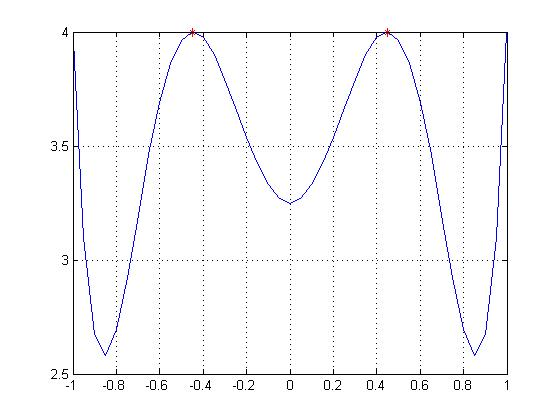
\includegraphics[width=10cm]{figures/GRAFICA1.jpg}\\
 Figura 1.1 \ Ejemplo 3 
\par\end{center}

Por lo tanto $\xi^{*}$ es $D$-�ptimo. 


\section{Dise�os de Bloqueos Completos Aleatorizados}

En cualquier experimento la variabilidad que surge de un factor perturbador
puede afectar los resultados. 


\subsubsection*{Factor Perturbador.}

Puede definirse como un factor del dise�o que probablemente tenga
un efecto sobre la respuesta pero en el que no existe inter�s espec�fico.

En ocasiones un factor perturbador es desconocido y no controlable
(se desconoce la existencia y puede tomar niveles variables mientras
se realiza el experimento).


\subsubsection*{La Aleatorizaci�n.}

Es una t�cnica de dise�o que se utiliza para protegerse contra factores
perturbadores.

en otros casos el factor perturbador es conocido pero no controlable.
Si por lo menos puede observarse el valor que asume el factor perturbador
en cada corrida del experimento, es posible hacer la compensaci�n
correspondiente en el an�lisis estad�stico mediante el uso del an�lisis
de covarianza.

Cuando la fuente de variabilidad perturbadora es conocida y controlable,
puede usarse una t�cnica de dise�o llamada formaci�n de bloques para
eliminar de manera sistem�tica su efecto sobre las comparaciones estad�sticas
entre los tratamientos.

La formaci�n de bloques es una t�cnica de dise�o en extremo importante
que se utiliza ampliamente en la experimentaci�n industrial.

El error experimental reflejar� tanto el error aleatorio como la variabilidad
entre los ejemplares de prueba.

El objetivo ser�a hacer el error experimental tan peque�o como fuera
posible (eliminar del error experimental la variabilidad entre los
ejemplares de prueba).

Un dise�o para lograr lo anterior es el dise�o de bloques completos
aleatorizados (RCBD, Randomized Complete Block Design). La palabra
``Completos'' indica que cada bloque (ejemplar de prueba) contiene
todos los tratamientos.
\begin{itemize}
\item Ejemplos de factor perturbador: Materia prima, personas, tiempo, etc.
\end{itemize}
La unidad experimental es el total de corridas en un experimento.


\subsection*{An�lisis Estad�stico Del Dise�o de Bloques Completos Aleatorizados}

Supongase que se tienen $a$ tratamientos que van a compararse y $b$
bloques.

Hay una observaci�n por tratamiento en cada bloque, y el orden en
que se corren los tratamientos dentro de cada bloque se determinan
al azar.

$\begin{array}{cccc}
\mbox{Bloque\mbox{ 1}} & \mbox{Bloque 2} & \mbox{} & \mbox{Bloque b}\\
y_{11} & y_{12} & y_{1j} & y_{1b}\\
y_{21} & y_{22} & y_{2j} & y_{2b}\\
y_{i1} & y_{i2} & y_{ij} & y_{ib}\\
\vdots & \vdots & \vdots & \vdots\\
y_{a1} & y_{a2} & y_{aj} & y_{ab}
\end{array}$

El dise�o estad�stico de RCBD puede escribirse de varias maneras.
El tradicional es el modelo de los efectos:

$y_{ij}=\mu+\tau_{i}+\beta_{j}+\epsilon_{ij}\begin{cases}
i & =1,2,\ldots,a\\
j & =1,2,\ldots,b
\end{cases}$

$Y_{ki}=a_{ki}+f(X_{ki})^{\tau}\beta$ con $i=1,2,\ldots,b$ y $k=1,2,\ldots,a$

$f(X_{ki})=[f_{1}(X_{ki}),\ldots,f_{a}(X_{ki})]$

donde $\mu$ es la media global, $\tau_{i}$ es el efecto del tratamiento
$i-\acute{e}simo$, $\beta_{j}$ es el efecto del bloque $j-\acute{e}simo$,
y $\epsilon_{ij}$ es el t�rmino del error $NID(O,\sigma^{2})$ usual.

Se considerar� inicialmente que los tratamientos y los bloques son
factores fijos.

El modelo de los efectos para el RCBD es un modelo especificado, los
efectos de los tratamientos y los bloques se consideran por lo general
como desviaciones de la media global por lo que:

${\displaystyle {\textstyle {\textstyle {\displaystyle \sum_{i=1}^{a}{\displaystyle \tau_{i}=0}}}}}$
y ${\displaystyle \sum_{j=1}^{b}}{\displaystyle \beta_{j}=0}$

Tambi�n es posible usar un modelo de las medias para el RCBD:

$y_{ij}=\mu_{ij}+\epsilon_{ij}\begin{cases}
i & =1,2,\ldots,a\\
j & =1,2,\ldots,b
\end{cases}$

Donde $\mu_{ij}=\mu+\tau_{i}+\beta_{j}$

En un experimento en el que se use RCBD, el inter�s se encuentra en
probar la igualdad de las medias de los tratamiento. Por lo tanto,
las hip�tesis de inter�s son:

$H_{0}:\mu_{1}=\mu_{2}=\ldots=\mu_{a}$

$H_{1}:\mbox{ Al menos una \ensuremath{\mu_{i}\neq\mu_{j}}}$

Puesto que la media del tratamiento $i-\acute{e}simo$ es $\mu_{i}=\frac{1}{b}{\displaystyle \sum_{j=1}^{b}(\mu+\tau_{i}+\beta_{j})=\mu+\tau_{i}}$

Otra forma de escribir las hip�tesis en t�rminos de los efectos de
los tratamientos es:

$H_{0}:\tau_{1}=\tau_{2}=\ldots=\tau_{a}=0$

$H_{1}:\mbox{ \ensuremath{\tau_{i}\neq0}Para al menos una \ensuremath{i}}$

Sea $y_{i.}$ el total de observaciones hechas bajo el tratamiento
$i$.

$y_{.j}$ el total de observaciones del bloque $.j$

$y_{..}$el gran total de las observaciones.

$N=ab$ el n�mero total de observaciones. expresado matem�ticamente.

$y_{i.}={\displaystyle \sum_{j=1}^{b}y_{ij}}$ con $i=1,2,\ldots,a$

$y_{.j}={\displaystyle \sum_{i=1}^{a}y_{ij}}$ con $j=1,2,\ldots,b$

$y_{..}={\displaystyle \sum_{i=1}^{a}{\displaystyle \sum_{j=1}^{b}y_{ij}={\displaystyle \sum_{i=1}^{a}y_{i.}={\displaystyle \sum_{j=1}^{b}y_{.j}}}}}$

De manera similar, $\bar{y_{i}}$es el promedio de las observaciones
hechas bajo el tratamiento $i$

$y$ es el promedio de las observaciones del bloque $j$.

$\bar{y}_{..}$es el gran promedio total de las observaciones.

es decir $\bar{y}_{i.}=\frac{y_{i.}}{b}$; $\bar{y}=\frac{y_{.j}}{a}$;
$\frac{\bar{y}_{..}}{N}$

La suma de cuadrados total corregida puede expresarse como:

$\begin{array}{ccc}
{\displaystyle \sum_{i=1}^{a}}{\displaystyle \sum_{j=1}^{b}(y_{ij}-\bar{y}_{..})^{2}} & = & \sum_{i=1}^{a}{\displaystyle \sum_{j=1}^{b}[(\bar{y}_{i.}-\bar{y}_{..})+}\bar{y}_{.j}-\bar{y}_{..})+(\bar{y}_{ij}-\bar{y}_{i.}-\bar{y}_{.j}+\bar{y}_{..})]^{2}\\
 & = & b{\displaystyle \sum_{i=1}^{a}(\bar{y}_{i.}-\bar{y}_{..})^{2}+a\sum_{j=1}^{b}(\bar{y}_{.j}-\bar{y}_{..})^{2}+\sum_{i=1}^{a}{\displaystyle \sum_{j=1}^{b}(\bar{y}_{ij}-\bar{y}_{.j}-\bar{y}_{i.}+\bar{y}_{..})^{2}}}
\end{array}${*}

Al expresar simb�licamente las sumas de cuadrados, se tiene: $SS_{T}=SS_{Tratamientos}+SS_{Bloques}+SS_{E}$
{*}'

Puesto que hay $N$ observaciones, $a$ tratamientos y $b$ bloques,
$SS_{T}$ tiene $N-1$ grados de libertad, $SS_{Tratamientos}$ tiene
$a-1$ grados de libertad y $SS_{Bloques}$tiene $b-1$ grados de
libertad.

Como $SS_{E}=SS_{T}-(SS_{Tratamientos}+SS_{Bloques})$ y $N=ab$ entonces
$SS_{E}$ tiene $ab-1-(a-1)-(b-1)=(a-1)(b-1)$ grados de libertad.

Como la suma de los grados de libertad del lado derecho es igual al
total del lado izquierdo de {*}', por lo tanto, al establecer los
supuestos de normalidad usuales para los errores, puede usarse el
Teorema de Cochran para demostrar que $\frac{SS_{Tratamientos}}{\sigma^{2}}$;
$\frac{SS_{Bloques}}{\sigma^{2}}$y $\frac{SS_{E}}{\sigma^{2}}$ son
variables aleatorias $ji-cuadradas$ con distribuciones independientes.

Cada suma de cuadrados dividida por sus grados de libertad es un cuadrado
medio.

Puede demostrarse que el valor esperado de los cuadrados medios, si
los tratamientos y los bloques son fijos, es:

$E(MS_{Tratamientos})=\sigma^{2}+\frac{b{\displaystyle \sum_{i=1}^{a}\tau_{i}^{2}}}{a-1}$

$E(MS_{Bloques})=\sigma^{2}+\frac{a{\displaystyle \sum_{j=1}^{b}}\beta_{j}^{2}}{b-1}$

$E(MS_{E})=\sigma^{2}$

Por lo tanto, para probar la igualdad de las medias de los tratamientos,
se usar�a el estad�stico de prueba:

$F_{0}=\frac{MS_{Tratamientos}}{MS_{E}}$

Que se distribuye como $F_{a-1,(a-1)(b-1)}$si la hip�tesis nula es
verdadera.

La regi�n cr�tica es la cola superior de la distribuci�n $F$, y $H_{0}$se
rechaza si $F_{0}>F_{a,a-1,(a-1)(b-1)}$

Tambi�n podr�a haber inter�s en comparar las medidas de los bloques
porque, en caso de que la diferencia entre estas medias no sea considerables,
quiz� no sea necesaria la formaci�n de bloques en experimentos futuros.

Por los cuadrados medios esperados, aparentemente la hip�tesis $H_{0}:\beta_{j}=0$
puede probarse comparando el estad�stico $F_{0}=\frac{MS_{Bloques}}{MS_{E}}$
con $F_{a,b-1,(a-1)(b-1)}$
\begin{description}
\item [{Recuerde:}] la aleatorizaci�n s�lo se ha aplicado a los tratamientos
dentro de los bloques, es decir, los bloques representan una restricci�n
sobre la aleatorizaci�n.
\end{description}
�Qu� efecto tiene lo anterior sobre el estad�stico $F_{0}=\frac{MS_{Bloques}}{MS_{E}}$?

\label{Box, Hunter =000026 Hunter} se�alan que la prueba $F$del
an�lisis de varianza com�n puede justificarse exclusivamente con base
a la aleatorizaci�n, si el uso supuesto de normalidad (debido a la
restricci�n sobre la aleatorizaci�n). Pero si los errores son $NID(O,\sigma^{2})$,
puede usarse $F_{0}=\frac{MS_{Bloques}}{MS_{E}}$ para comparar las
medias de los bloques.

\label{Anderson =000026 McLean} argumentan que la restricci�n sobre
la aleatorizaci�n impide que este estad�stico sea una prueba significativa
para comparar las medias de los bloques y que este cociente $F$ es
en realidad una prueba de la igualdad de las medias de los bloques
m�s la restricci�n sobre la aleatorizaci�n ( a la que le llaman error
de la restricci�n).

Entonces, �Qu� se hace en la pr�ctica?

Debido a que con frecuencia el supuesto de normalidad es cuestionable,
considerar $F_{0}=\frac{MS_{Bloques}}{MS_{E}}$ como una prueba $F$
exacta para la igualdad de las medias de los bloques no es una buena
pr�ctica general.

Por lo anterior esta prueba $F$ no se incluye en la tabla del an�lisis
de varianza.

Sin embargo, como un procedimiento aproximado para investigar el efecto
de la variable formaci�n de bloques, examinar el cociente $\frac{MS_{Bloques}}{MS_{E}}$
es razonable. Si este cociente es muy grande implica que el factor
formaci�n de bloques tiene un efecto considerable y que la reducci�n
del ruido obtenida, por la formaci�n de bloques probablemente fue
�til para mejorar la precisi�n de la comparaci�n de las medias de
los tratamientos.

El procedimiento suele resumirse en un esquema de an�lisis de varianza,
como el que se muestra en la tabla {*}{*} (los c�lculos se realizar�n
con un paquete de software de estad�stica).

Sin embargo es posible obtener formulas de c�lculo manual para la
suma de cuadrados para los elementos de la ecuaci�n {*} expres�ndolos
en t�rminos de los totales de los tratamientos y los bloques. �stas
son:

$SS_{T}={\displaystyle \sum_{i=1}^{a}}{\displaystyle \sum_{j=1}^{b}y_{ij}^{2}-\frac{y_{..}^{2}}{N}}$

$SS_{Tratamientos}=\frac{1}{b}{\displaystyle \sum_{i=1}^{a}}y_{i.}^{2}{\displaystyle -\frac{y_{..}^{2}}{N}}-$

$SS_{Bloques}=\frac{1}{a}{\displaystyle \sum_{j=1}^{b}y_{.j}^{2}-\frac{y_{..}^{2}}{N}}$

y $SS_{E}=SS_{T}-SS_{Tratamientos}-SS_{Bloques}$

\begin{table}
\protect\caption{An�lisis de Varianza de un Dise�o de Bloques Completos Aleatorizados.
{*}{*}}


\begin{tabular}{|c|c|c|c|c|}
\hline 
Fuente de Variaci�n & Suma de Cuadrados & Grados de Libertad & Cuadrado Medio & $F_{0}$\tabularnewline
\hline 
\hline 
Tratamientos & $SS_{Tratamientos}$ & $a-1$ & $\frac{SS_{Tratamientos}}{a-1}$ & $\frac{MS_{Tratamientos}}{MS_{E}}$\tabularnewline
\hline 
Bloques & $SS_{Bloques}$ & $b-1$ & $\frac{SS_{Bloques}}{b-1}$ & \tabularnewline
\hline 
Error & $SS_{E}$ & $(a-1)(b-1)$ & $\frac{SS_{E}}{(a-1)(b-1)}$ & \tabularnewline
\hline 
Total & $SS_{T}$ & $N-1$ &  & \tabularnewline
\hline 
\end{tabular}
\end{table}



\section{Experimentos Con Factores Aleatorios}


\subsubsection*{Factores Fijos.}

Quiere decir que los niveles de los factores usados por el experimentador
son los niveles de inter�s espec�ficos. 
\begin{itemize}
\item Ejemplo: si se investigan $3$ tipos de materiales, las conclusiones
son v�lidas solo para esos tipos espec�ficos de materiales.
\end{itemize}
Una variante de lo anterior ocurre cuando el factor o factores son
cuantitativos.

Cuando se trabaja con un efecto fijo, se dice que el espacio inferencial
del experimento es el conjunto espec�fico de los niveles de los factores
investigados.

En algunas situaciones experimentales, los niveles de los factores
se eligen al azar de una poblaci�n m�s grande de niveles posibles,
no s�lo de los que se usaron en el dise�o experimental. En esta situaci�n
se dice que se trata de un factor aleatorio.

Se empieza con una situaci�n simple, un experimento con un solo factor
en el que el factor es aleatorio y se usa esto para introducir el
modelo de efectos aleatorios para el an�lisis de varianza y los componentes
de varianza. Los factores aleatorios ocurren normalmente en experimentos
factoriales, as� como en otros de tipos de experimentos.


\subsubsection*{Modelo Con Efectos Aleatorios.}

Es com�n que un experimentador est� interesado en un factor que tiene
un gran n�mero de posibles niveles. Cuando el experimentador selecciona
aleatoriamente $a$ de estos niveles de la poblaci�n de los niveles
del factor, entonces se dice que el factor es aleatorio.

Puesto que los niveles del factor utilizados en el experimento se
eligen al azar, se hacer inferencias acerca de la poblaci�n completa
de los niveles del factor.

Se supone que la poblaci�n de los niveles del factor es de tama�o
infinito o bien lo suficientemente grande para considerarla infinita.
No es frecuente encontrar situaciones en la que la poblaci�n de los
niveles del factor sea lo suficientemente peque�a para encontrar el
enfoque de una poblaci�n finita.

El modelo estad�stico lineal es:

$y_{ij}=\mu+\tau_{i}+\epsilon_{ij}\begin{cases}
i & =1,2,\ldots,a\\
j & =1,2,\ldots,n
\end{cases}${*}

Donde $\tau_{i}$ y $\epsilon_{ij}$ son variables aleatorias. si
$\tau_{i}$ tiene varianza $\sigma_{\tau}^{2}$ y es independiente
de $\epsilon_{ij}$ la varianza de cualquier observaci�n es: 

$E(y_{ij})=\mu$ y $v(y_{ij})=\sigma_{\tau}^{2}+\sigma^{2}$

A las varianzas $\sigma_{\tau}^{2}$ y $\sigma^{2}$ se les llama
los componentes de varianza y al modelo de la ecuaci�n {*} se le llama
modelo de los efectos aleatorios o de los componentes de la varianza.

Para probar hip�tesis en este modelo se requiere que las $\left\{ \epsilon_{ij}\right\} $sean
$NID(O,\sigma^{2})$, que las $\left\{ \tau_{i}\right\} $ sean $NID(O,\sigma_{\tau}^{2})$
y que $\tau_{i}$ y $\epsilon_{ij}$ sean independientes.

La suma de cuadrados identidad $SS_{T}=SS_{Tratamientos}+SS_{E}$
sigue siendo valida.

Es decir, se hace la partici�n de la variabilidad total en las observaciones
en un componente que mide la variaci�n entre los tratamientos ($SS_{Tratamientos}$)
en un componente dentro de los tratamientos ($SS_{E}$).

Probar hip�tesis acerca de los efectos de tratamientos individuales
no tiene sentido, por lo que en su lugar se prueban hip�tesis acerca
del componente de la varianza $\sigma_{\tau}^{2}$.

$H_{0}:\sigma_{\tau}^{2}=0$

$H_{1}:\sigma_{\tau}^{2}>0$

entonces si $\sigma_{\tau}^{2}=0$, todos los tratamientos son id�nticos,
pero si $\sigma_{\tau}^{2}>0$, existe variabilidad entre los tratamientos. 

Como anteriormente

$\frac{SS_{E}}{\sigma^{2}}$ se distribuye como $ji-cuadrado$ con
$N-a$ grados de libertad y, bajo la hip�tesis nula $(\sigma_{\tau}^{2}=0)$

$\frac{SS_{Tratamientos}}{\sigma^{2}}$ se distribuye como $ji-cuadrada$
con $a-1$ grados de libertad

Ambas variables aleatorias son independientes, por lo tanto bajo $\sigma_{\tau}^{2}=0$,
el cociente

$F_{0}=\frac{\frac{SS_{Tratamientos}}{a-1}}{\frac{SS_{E}}{N-a}}=\frac{MS_{Tratamientos}}{MS_{E}}$

Se distribuye como $F$ con $a-1$ y $N-a$ grados de libertad.

Ahora 

$\begin{array}{ccc}
E(MS_{Tratamientos}) & = & \frac{1}{a-1}E(SS_{Tratamientos})\\
E(MS_{Tratamientos}) & = & \frac{1}{a-1}E({\displaystyle \sum_{i=1}^{a}(\frac{y_{i.}^{2}}{n}-\frac{y_{..}^{2}}{N})}
\end{array}$

$\begin{array}{ccc}
E(MS_{Tratamientos}) & = & \frac{1}{a-1}E[\frac{1}{n}{\displaystyle \sum_{i=1}^{a}({\displaystyle \sum_{j=1}^{a}(\mu+\tau_{i}+\epsilon_{ij})^{2}-}}\frac{1}{N}({\displaystyle \sum_{i=1}^{a}{\displaystyle \sum_{j=1}^{n}(\mu+\tau_{i}+\epsilon_{ij})^{2}]}}\end{array}$

Cuando se eleva al cuadrado y se toma la funci�n esperanza de las
cantidades entre corchetes, se observa que $\tau_{i}^{2}$ es reemplazada
por $\sigma_{\tau}^{2}$ $E(\tau_{i})=0$. Adem�s $\epsilon_{i.}^{2},\epsilon_{..}^{2}$
y ${\displaystyle \sum_{i=1}^{a}{\displaystyle \sum_{j=1}^{n}\tau_{i}^{2}}}$
son reemplazadas por $n\sigma^{2},an\sigma^{2}$ y $an^{2}\sigma^{2}$,
respectivamente y todos los productos cruzados que incluyen a $\tau_{i}$
y $\epsilon_{ij}$ tienen valor esperado cero. Esto lleva a:

$E(MS_{Tratamientos})=\frac{1}{a-1}[N\mu^{2}+N\sigma_{\tau}^{2}+a\sigma^{2}-n\mu^{2}-n\sigma_{\tau}^{2}-\sigma^{2}$
� $E(MS_{Tratamientos})=\sigma^{2}+n\sigma_{\tau}^{2}$

De manera similar, puede demostrarse que

$E(MS_{E})=\sigma^{2}$

Por los cuadrados medios esperados, se observa que bajo $H_{0}$tanto
el numerado como el denominador del estad�stico de prueba ($F_{0}=\frac{MS_{Tratamientos}}{MS_{E}}$)
son estimadores insesgados de $\sigma$$^{2}.$

Mientras que bajo $H_{1}$el valor esperado del numerado es mayor
que el del denominador. Por lo tanto $H_{0}$deber� rechazarse para
los valores de $F_{0}$que sean muy grandes.

$H_{0}$ se rechaza si $F_{0}>F_{a,a-1,N-a}$

El procedimiento de c�lculo y el an�lisis de la tabla de varianza
del modelo de efectos aleatorios son id�nticos a los que se utilizaron
en el caso de efectos fijos. Sin embargo las conclusiones son muy
diferentes, ya que se aplican a la poblaci�n completa de los tratamientos.

Por lo general habr� inter�s en estimar los componentes de la varianza
($\sigma^{2}$ y $\sigma_{\tau}^{2}$) del modelo.

Al procedimiento que se usa para estimar $\sigma^{2}$ y $\sigma_{\tau}^{2}$,
se le llama m�todo del an�lisis de varianza, ya que hace uso de las
lineas de la tabla del an�lisis de varianza.

El procedimiento consiste en igualar los cuadrados medios esperados
con sus valores observados en la tabla del an�lisis de varianza y
despejar los componentes de la varianza.

Al igualar los cuadrados medios observados con los esperados en el
modelo de efectos aleatorios con un solo factor, se obtiene

$MS_{Tratamientos}=\sigma^{2}+n\sigma_{\tau}^{2}$ y $MS_{E}=\sigma^{2}$

Por lo tanto, los estimadores de los componentes de la varianza son 

$\hat{\sigma}^{2}=MS_{E}$ y $\hat{\sigma}_{\tau}^{2}=\frac{MS_{Tratamientos}-MS_{E}}{n}$

Para tama�os de las muestras desiguales, se reemplaza $n$ en {*}
con

$n_{0}=\frac{1}{a-1}[{\displaystyle \sum_{i=1}^{a}n_{i}-\frac{{\displaystyle \sum_{i=1}^{a}n_{i}^{2}}}{{\displaystyle \sum_{i=1}^{a}n_{i}}}]}=\frac{N-\frac{{\displaystyle \sum_{i=1}^{a}n_{i}^{2}}}{N}}{a-1}$

En el m�todo del an�lisis de varianza para estimar los componentes
de la varianza no se requiere el supuesto de normalidad.

El m�todo produce estimadores $\sigma^{2}$y $\sigma_{\tau}^{2}$,
que son los mejores estimadores cuadr�ticos insesgados (estos estimadores
tienen m�nima varianza).

Ocasionalmente, el m�todo del an�lisis de varianza produce una estimaci�n
negativa de uno de los componentes de la varianza. Evidentemente,
los componentes de la varianza son por definici�n no negativos, por
lo que la estimaci�n negativa de un componente de la varianza se considera
con un cierta preocupaci�n.

Un curso de acci�n es aceptar la estimaci�n negativa y usarla como
evidencia de que el verdadero valor del componente de la varianza
es cero (aunque esto adolece dificultades te�ricas). usar cero en
lugar de la estimaci�n negativa puede alterar las propiedades estad�sticas
de otras estimaciones.

Otra alternativa es volver a estimar el componente de la varianza
utilizando un m�todo que produzca siempre estimaciones no negativas.

y otra alternativa es considerar la estimaci�n negativa como evidencia
de que el modelo lineal supuesto es incorrecto y examinar de nuevo
el problema.


\section{Modelo Mixto Con Dos Factores}

Se considera ahora la situaci�n en que uno de los factores $A$ este
fijo y el otro, $B$, es aleatorio. Se le llama an�lisis de varianza
del modelo mixto. El modelo estad�stico lineal es:

$y_{ijk}=\mu+\tau_{i}+\beta_{j}+(\tau\beta)_{ij}+\epsilon_{ijk}\begin{cases}
i & =1,2,\ldots,a\\
j & =1,2,\ldots,b\\
k & =1,2,\ldots,n
\end{cases}$

Donde

$\tau_{i}$ es un efecto fijo.

$\beta_{j}$ es un efecto aleatorio.

$(\tau\beta)_{ij}$ es un efecto aleatorio (se supone).

$\epsilon_{ijk}$ es un error aleatorio.

Se supone que las $\left\{ \tau_{i}\right\} $son efectos fijos tales
que ${\displaystyle \sum_{i=1}^{a}}\tau_{i}=0$ y que $\beta_{j}$
es una variable aleatoria $NID(O,\sigma_{\beta}^{2})$.

El efecto de la interacci�n $(\tau\beta)_{ij}$, es una variable aleatoria
normal con media $0$ y varianza $(\frac{a-1}{a})\sigma_{\tau\beta}^{2}$

La operaci�n suma del componente de la interacci�n en el rando del
factor fijo es igual a cero ${\displaystyle \sum_{i=1}^{a}}(\tau\beta)_{ij}=(\tau\beta)_{.j}=0$
con $j=1,2,\ldots,b$

Esta restricci�n implica que algunos elementos de la interacci�n en
diferentes niveles del factor fijo no son independientes, puede demostrarse
que:

$Cov[(\tau\beta)_{ij},(\tau\beta)_{i'j}]=-\frac{1}{a}\sigma_{\tau\beta}^{2}$
para $i\neq i'$

la $Cov$ entre $(\tau\beta)_{ij}$ y $(\tau\beta)_{ij'}$para $j\neq j'$
es cero, y el error aleatorio $\epsilon_{ijk}$ es $NID(O,\sigma^{2})$

Puesto que la suma de los efectos de la interacci�n en los niveles
del factor fijo es igual a cero, a esta versi�n del modelo mixto se
le llama modelo restringido.

En este modelo la varianza de $(\tau\beta)_{ij}$ se define como $(\frac{a-1}{a})\sigma_{\tau\beta}^{2}$
en vez de como $\sigma_{\tau\beta}^{2}$ para simplificar los cuadrados
medios esperados. El supuesto $(\tau\beta)_{.j}=0$ tambi�n tiene
un efecto sobre los cuadrados medios esperados, los cuales se pueden
demostrar que son:

$E(MS_{A})=\sigma^{2}+n\sigma_{\tau\beta}^{2}+\frac{bn{\displaystyle \sum_{i=1}^{a}\tau_{i}^{2}}}{a-1}$

$E(MS_{B})=\sigma^{2}+an\sigma_{\beta}^{2}$

$E(MS_{AB})=\sigma^{2}+an\sigma_{\tau\beta}^{2}$

y $E(MS_{E})=\sigma^{2}$

Por lo tanto, el estad�stico de prueba aprobado para probar que las
media de los efectos del factor fijo son iguales, o $H_{0}:\tau_{i}=0$
es $F_{0}=\frac{MS_{A}}{MS_{AB}}$ que tiene la distribuci�n de referencia
$F_{a-1,(a-1)(b-1)}$

Para probar $H_{0}:\sigma_{\beta}^{2},$ es el estad�stico de prueba
es $F_{0}=\frac{MS_{B}}{MS_{E}}$

Con la distribuci�n de referencia $F_{b-1,ab(n-1)}$

Por �ltimo, para probar la hip�tesis de la interferencia $H_{0}:\sigma_{\tau\beta}^{2}=0$

$F_{0}=\frac{MS_{AB}}{MS_{E}}$

Que tiene la distribuci�n de frecuencia $F_{(a-1)(b-1),ab(n-1)}$

En el modelo mixto es posible estimar los efectos del factor fijo
como: $\hat{\mu}=\bar{y}$ y $\hat{\tau_{i}}=\bar{y}_{i..}-\bar{y}_{...}$
para $i=1,2,\ldots,a$

Los componentes de la varianza $\sigma_{\beta}^{2}$, $\sigma_{\tau\beta}^{2}$
y $\sigma^{2}$ pueden estimarse aplicando el m�todo del an�lisis
de varianza. de {*} quedan:

$\sigma^{2}=\frac{MS_{B}-MS_{E}}{an}$

$\sigma_{\tau\beta}^{2}=\frac{MS_{AB}MS_{E}}{n}$

y $\sigma^{2}=MS_{E}$

Este enfoque general puede emplearse para estimar los componentes
de la varianza en cualquier modelo mixto.


\section{Dise�o Factorial de Dos Factores Aleatorios}

Suponga que se tienen dos factores, $A$ y $B$, y que ambos tienen
un gran n�mero de niveles de inter�s. Se escogen al azar $a$ niveles
del factor $A$ y $b$ niveles del factor $B$. si el experimento
se hace con $n$ r�plicas las observaciones pueden representarse con
el modelo lineal:

$y_{ijk}=\mu+\tau_{i}+\beta_{j}+(\tau\beta)_{ij}+\epsilon_{ijk}\begin{cases}
i & =1,2,\ldots,a\\
j & =1,2,\ldots,b\\
k & =1,2,\ldots,n
\end{cases}$

Donde todos los par�metros del modelo, $\tau_{i}$,$\beta_{j}$,$(\tau\beta)_{ij}$
y$\epsilon_{ijk}$, son variables aleatorias independientes.

Tambi�n se supondr� que las variables aleatorias $\tau_{i}$,$\beta_{j}$,$(\tau\beta)_{ij}$
y$\epsilon_{ijk}$ siguen una distribuci�n normal con media cero y
varianzas $v(\tau_{i})=\sigma$, $v(\beta_{j})=\sigma_{\beta}^{2}$,
$v[(\tau\beta)_{ij}]=\sigma_{\tau\beta}^{2}$ y $v(\epsilon_{ijk})=\sigma^{2}$
Por lo tanto.

$v(y_{ijk})=\sigma_{\tau}^{2}+\sigma_{\beta}^{2}+\sigma_{\tau\beta}^{2}+\sigma^{2}$
y $\sigma_{\tau}^{2}$, $\sigma_{\beta}^{2}$, $\sigma_{\tau\beta}^{2}$
y $\sigma^{2}$son los componentes de la varianza.

Las hip�tesis que quieren probarse son $H_{0}:\sigma_{\tau}^{2}=0$
y $H_{0}:\sigma_{\beta}^{2}=0$

Los c�lculos num�ricos del an�lisis de varianza ($SS_{A}$, $SS_{B}$,
$SS_{T}$, $SS_{E}$) se calculan como en el caso de efectos fijos.
Para formar los estad�sticos de prueba, deben examinarse los cuadrados
medios esperados, puede demostrarse que:

$E(MS_{A})=\sigma^{2}+n\sigma_{\tau\beta}^{2}+bn\sigma_{\tau}^{2}$

$E(MS_{B})=\sigma^{2}+n\sigma_{\tau\beta}^{2}+an\sigma_{\beta}^{2}$

$E(MS_{AB})=\sigma^{2}+n\sigma_{\tau\beta}^{2}$

y $E(MS_{E})=\sigma^{2}$

Por los cuadrados medios esperados se observa que el estad�stico apropiado
para probar la hip�tesis de que no hay interacci�n, $H_{0}:\sigma_{\tau\beta}^{2}=0$
es $F_{0}=\frac{MS_{AB}}{MS_{E}}$

Ya que bajo $H_{0}$ tanto el numerador como el denominador de $F_{0}$tienen
valor esperado $\sigma^{2}$, y solo si $H_{0}$es falsa $E(MS_{AB})$
es mayor que $E(MS_{E})$. El cociente $F_{0}$ se distribuye como
$F_{(a-1),ab(n-1)}$ de manera similar para probar $H_{0}:\sigma_{\tau}^{2}=0$
se usar�a $F_{0}=\frac{MS_{A}}{MS_{Ab}}$

Que se distribuye como $F_{a-1,(a-1)(b-1)}$ y para probar $H_{0}:\sigma_{\beta}^{2}=0$
el estad�stico es $F_{0}=\frac{MS_{B}}{MS_{AB}}$

Que se distribuye como $F_{b-1,(a-1)(b-1)}$

Los componentes de la varianza pueden estimarse con el m�todo del
an�lisis de varianza

$\hat{\sigma}^{2}=MS_{E}$

$\hat{\sigma}_{\tau\beta}^{2}=\frac{MS_{AB}-MS_{E}}{n}$

$\hat{\sigma}_{\beta}^{2}=\frac{MS_{E}-MS_{AB}}{an}$

$\hat{\sigma}_{\tau}^{2}=\frac{MS_{A}-MS_{AB}}{bn}$


\clearemptydoublepage

%%%% BLOCK 3\partgreen{[}{]}{\textbf{M}eta} 
\chapter{\textcolor{blue}{Dise�os �ptimos en la presencia de efectos de bloques
aleatorios}}

\label{AB2}

%recuperar numeracion arabica%\global\long\def\thechapter{\arabic{chapter}}



\lettrine[lines=4,loversize=-0.1,lraise=0.1,lhang=.2]{P}{}{ara un modelo lineal en la presencia de efectos de bloques aleatorios
se describe la situaci�n donde se tienen $b$ bloques, cada uno con
$m_{i}$ observaciones. Por lo tanto,la $j$-�sima observaci�n $Y_{ij}$
al bloque $i$ se puede escribir como\\
 
\begin{equation}
Y_{ij}=\gamma_{i}+\beta_{0}+\mathbf{f}(\mathrm{x}_{ij})^{\top}\boldsymbol{\beta}+\epsilon_{ij}
\end{equation}
\\
 donde $\mathrm{x}_{ij}$ son los puntos experimentales, $j=1,...,m_{i}$,
$\boldsymbol{f}=(f_{1},...,f_{p})^{\top}$ es un conjunto de funciones
(conocidas) de regresi�n y $\beta_{0}\in\mathbb{R}$, $\boldsymbol{\beta}=(\beta_{1},...,\beta_{p})^{\top}$
son los par�metros desconocidos. $f$ puede ser la funci�n identidad
para regresi�n lineal simple.\\
}

El t�rmino $\gamma_{i}$ es el efecto del $i$-�simo bloque aleatorio
con $E(\gamma_{i})=0$ y $Var(\gamma_{i})=\sigma_{\gamma}^{2}$. Los
errores de observaci�n aleatorio $\epsilon_{ij}$ se supone que son
homoscedasticos, $E(\epsilon_{ij})=0$, $Var(\epsilon_{ij})=\sigma^{2}$
y $Cov(\gamma_{i},\epsilon_{ij})=0$. El an�lisis adicional depender�
del cociente de varianza $d=\sigma_{\gamma}^{2}/\sigma^{2}$ . Nos
centraremos en los par�metros de la poblaci�n $\theta=(\beta_{0},\boldsymbol{\beta}^{\top})^{\top}$.
Asumiremos que el n�mero de observaciones por bloque es constante,
es decir, $m_{i}=m$.\\


Denotemos por $\boldsymbol{Y}_{i}=(Y_{i1},...,Y_{im})^{\top}$ el
vector de observaciones para el bloque $i$. La matriz de covarianza
correspondiente $Cov(\boldsymbol{Y}_{i})=\sigma^{2}\boldsymbol{V}$
es completamente sim�trica, $\boldsymbol{V}=\boldsymbol{I}_{m}+d\boldsymbol{1}_{m}\boldsymbol{1}_{m}^{\top}$,
donde $\boldsymbol{I}_{m}$ indica la matriz identidad $m\times m$
y $\boldsymbol{1}_{m}$ es un vector de longitud $m$ con todas las
entradas iguales a uno. El efecto fijo individual de la matriz de
dise�o $\boldsymbol{X}_{i}=(\boldsymbol{1}_{m}\mid\boldsymbol{F}_{i})$
se puede descomponer en la primera columna de unos correspondiente
a la intersecci�n $\beta_{0}$ y la matriz de dise�o para el vector
de par�metros $\boldsymbol{\beta}$.\\


La inversa de $\boldsymbol{V}$ la podemos hallar mediante �lgebra
matricial\
\begin{equation}
\begin{aligned}\boldsymbol{V}^{-1} & =(\boldsymbol{I}_{m}+d\boldsymbol{1}_{m}\boldsymbol{1}_{m}^{\top})^{-1}\\
 & =\boldsymbol{I}-d^{\frac{1}{2}}\boldsymbol{1}_{m}(\boldsymbol{I}+d\boldsymbol{1}_{m}^{\top}\boldsymbol{I}\boldsymbol{1}_{m})^{-1}d^{\frac{1}{2}}\boldsymbol{1}_{m}^{\top}\\
 & =\boldsymbol{I}-d\boldsymbol{1}_{m}(\boldsymbol{I}+dm\boldsymbol{I})^{-1}\boldsymbol{1}_{m}^{\top}\\
 & =\boldsymbol{I}-d\boldsymbol{1}_{m}(\boldsymbol{I}(1+dm))^{-1}\boldsymbol{1}_{m}^{\top}\\
 & =\boldsymbol{I}-\frac{d}{1+dm}\boldsymbol{1}_{m}\boldsymbol{1}_{m}^{\top}
\end{aligned}
\end{equation}
\\


Luego, la matriz de informaci�n por bloque, utilizando $(2\ldotp2)$
queda $\boldsymbol{X}_{i}^{\top}\boldsymbol{V}^{-1}\boldsymbol{X}_{i}=\boldsymbol{X}_{i}^{\top}\boldsymbol{X}_{i}-\frac{d}{1+md}\boldsymbol{X}_{i}^{\top}\boldsymbol{1}_{m}\boldsymbol{1}_{m}^{\top}\boldsymbol{X}_{i}$
que es proporcional a la inversa de la matriz de varianza-covarianza
$Cov(\boldsymbol{\hat{\theta}}_{i})$ si $\boldsymbol{X}_{i}$ es
de rango completo. As\'{i} $\boldsymbol{\theta}$ es estimado sobre
una base por bloque

\begin{equation}
\begin{aligned}\boldsymbol{\hat{\theta}}_{i} & =(\boldsymbol{X}_{i}^{\top}\boldsymbol{V}^{-1}\boldsymbol{X}_{i})^{-1}\boldsymbol{X}_{i}^{\top}\boldsymbol{V}^{-1}\boldsymbol{Y}_{i}\\
 & =(\boldsymbol{X}_{i}^{\top}\boldsymbol{X}_{i})^{-1}\boldsymbol{X}_{i}^{\top}\boldsymbol{Y}_{i}
\end{aligned}
\end{equation}
\\


Sobre la base de la poblaci�n el mejor estimador lineal insesgado
se puede calcular como $\boldsymbol{\hat{\theta}}=\left({\displaystyle \sum_{i=1}^{b}\boldsymbol{X}_{i}^{\top}\boldsymbol{V}^{-1}\boldsymbol{X}_{i}}\right)^{-1}{\displaystyle \sum_{i=1}^{b}\boldsymbol{X}_{i}^{\top}\boldsymbol{V}^{-1}\boldsymbol{X}_{i}\boldsymbol{\hat{\theta}}_{i}}$
si $d$ es conocido. Entonces $Cov(\boldsymbol{\hat{\theta}})=\sigma^{2}\boldsymbol{M}_{d}^{-1}$,
donde $\boldsymbol{M}_{d}={\displaystyle \sum_{i=1}^{b}\boldsymbol{X}_{i}^{\top}\boldsymbol{V}^{-1}\boldsymbol{X}_{i}}$
es la matriz de informaci�n sobre la base de la poblaci�n. El sub\'{i}ndice
$d$ indica la dependencia del cociente de varianzas $d$. Como $\boldsymbol{M}_{d}={\displaystyle \sum_{i=1}^{b}\boldsymbol{X}_{i}^{\top}\boldsymbol{X}_{i}-\frac{d}{1+md}{\displaystyle \sum_{i=1}^{b}\boldsymbol{X}_{i}^{\top}\boldsymbol{1}_{m}\boldsymbol{1}_{m}^{\top}\boldsymbol{X}_{i}}}$.
\\
\\


La matriz de informaci�n particionada de acuerdo a $\beta_{0}$ y
$\boldsymbol{\beta}$, es \\
 
\begin{equation}
\begin{aligned}\boldsymbol{M}_{d} & ={\displaystyle \sum_{i=1}^{b}\boldsymbol{X}_{i}^{\top}\boldsymbol{X}_{i}-\frac{d}{1+md}{\displaystyle \sum_{i=1}^{b}\boldsymbol{X}_{i}^{\top}\boldsymbol{1}_{m}\boldsymbol{1}_{m}^{\top}\boldsymbol{X}_{i}}}\\
\\
 & ={\displaystyle \sum_{i=1}^{b}(\boldsymbol{1}_{m}\mid\boldsymbol{F}_{i})^{\top}(\boldsymbol{1}_{m}\mid\boldsymbol{F}_{i})-\frac{d}{1+md}{\displaystyle \sum_{i=1}^{b}(\boldsymbol{1}_{m}\mid\boldsymbol{F}_{i})^{\top}\boldsymbol{1}_{m}\boldsymbol{1}_{m}^{\top}(\boldsymbol{1}_{m}\mid\boldsymbol{F}_{i})}}\\
\\
 & ={\displaystyle \sum_{i=1}^{b}\begin{pmatrix}\boldsymbol{1}_{m}^{\top}\\
\\
\boldsymbol{F}_{i}^{\top}
\end{pmatrix}(\boldsymbol{1}_{m}\mid\boldsymbol{F}_{i})-\frac{d}{1+md}{\displaystyle \sum_{i=1}^{b}\begin{pmatrix}\boldsymbol{1}_{m}^{\top}\\
\\
\boldsymbol{F}_{i}^{\top}
\end{pmatrix}\boldsymbol{1}_{m}\boldsymbol{1}_{m}^{\top}(\boldsymbol{1}_{m}\mid\boldsymbol{F}_{i})}}\\
\\
 & ={\displaystyle \sum_{i=1}^{b}\begin{pmatrix}m & \boldsymbol{1}_{m}^{\top}\boldsymbol{F}_{i}\\
\\
\boldsymbol{F}_{i}^{\top}\boldsymbol{1}_{m} & \boldsymbol{F}_{i}^{\top}\boldsymbol{F}_{i}
\end{pmatrix}-\frac{d}{1+md}{\displaystyle \sum_{i=1}^{b}\begin{pmatrix}m\\
\\
\boldsymbol{F}_{i}^{\top}\boldsymbol{1}_{m}
\end{pmatrix}(m\mid\boldsymbol{1}_{m}^{\top}\boldsymbol{F}_{i})}}\\
\\
 & ={\displaystyle \sum_{i=1}^{b}\begin{pmatrix}m & \boldsymbol{1}_{m}^{\top}\boldsymbol{F}_{i}\\
\\
\boldsymbol{F}_{i}^{\top}\boldsymbol{1}_{m} & \boldsymbol{F}_{i}^{\top}\boldsymbol{F}_{i}
\end{pmatrix}-\frac{d}{1+md}{\displaystyle \sum_{i=1}^{b}\begin{pmatrix}m^{2} & m\boldsymbol{1}_{m}^{\top}\boldsymbol{F}_{i}\\
\\
\boldsymbol{F}_{i}^{\top}\boldsymbol{1}_{m}m & \boldsymbol{F}_{i}^{\top}\boldsymbol{1}_{m}\boldsymbol{1}_{m}^{\top}\boldsymbol{F}_{i}
\end{pmatrix}}}\\
\\
 & =\frac{1}{1+md}{\displaystyle \sum_{i=1}^{b}\begin{pmatrix}m+m^{2}d & \boldsymbol{1}_{m}^{\top}\boldsymbol{F}_{i}+md\boldsymbol{1}_{m}^{\top}\boldsymbol{F}_{i}\\
\\
\boldsymbol{F}_{i}^{\top}\boldsymbol{1}_{m}+md\boldsymbol{F}_{i}^{\top}\boldsymbol{1}_{m} & \boldsymbol{F}_{i}^{\top}\boldsymbol{F}_{i}+md\boldsymbol{F}_{i}^{\top}\boldsymbol{F}_{i}
\end{pmatrix}}\\
\\
\end{aligned}
\end{equation}
\[
-\frac{1}{1+md}{\displaystyle \sum_{i=1}^{b}\begin{pmatrix}dm^{2} & dm\boldsymbol{1}_{m}^{\top}\boldsymbol{F}_{i}\\
\\
d\boldsymbol{F}_{i}^{\top}\boldsymbol{1}_{m}m & d\boldsymbol{F}_{i}^{\top}\boldsymbol{1}_{m}\boldsymbol{1}_{m}^{\top}\boldsymbol{F}_{i}
\end{pmatrix}}
\]


\begin{equation}
\boldsymbol{M}_{d}=\frac{1}{1+md}\left(\begin{tabular}{c|c}
 \ensuremath{bm}  &  \ensuremath{{\displaystyle \sum_{i=1}^{b}\boldsymbol{1}_{m}^{T}\boldsymbol{F}_{i}}} \\
\hline \ensuremath{{\displaystyle \sum_{i=1}^{b}\boldsymbol{F}_{i}^{\top}\boldsymbol{1}_{m}}}  &  \ensuremath{(1+md){\displaystyle \sum_{i=1}^{b}\boldsymbol{F}_{i}^{\top}\boldsymbol{F}_{i}-d{\displaystyle \sum_{i=1}^{b}\boldsymbol{F}_{i}^{\top}\boldsymbol{1}_{m}\boldsymbol{1}_{m}^{\top}\boldsymbol{F}_{i}}}} 
\end{tabular}\right)
\end{equation}
\\
 \\


Si el inter�s est� en los efectos fijos $\boldsymbol{\beta}$ solamente,
entonces las reglas para invertir las correspondientes matrices de
informaci�n parcial particionadas $\boldsymbol{M}_{\boldsymbol{\beta},d}^{-1}=Cov(\boldsymbol{\hat{\beta}})/\sigma^{2}$
es igual a\\
 
\begin{equation}
\boldsymbol{M}_{\boldsymbol{\beta},d}={\displaystyle \sum_{i=1}^{b}\boldsymbol{F}_{i}^{\top}\boldsymbol{F}_{i}-\frac{d}{1+md}{\displaystyle \sum_{i=1}^{b}\boldsymbol{F}_{i}^{\top}\boldsymbol{1}_{m}\boldsymbol{1}_{m}^{\top}\boldsymbol{F}_{i}-\frac{1}{bm}\ \frac{1}{1+md}\left({\displaystyle \sum_{i=1}^{b}\boldsymbol{F}_{i}^{\top}\boldsymbol{1}_{m}}\right)\left({\displaystyle \sum_{i=1}^{b}\boldsymbol{1}_{m}^{\top}\boldsymbol{F}_{i}}\right)}}
\end{equation}
\\
 \\
 Tambi�n consideramos los modelos l\'{i}mites para $d=0$ y $d\rightarrow\infty$,
respectivamente: Para $d=0$ obtenemos los modelos de efectos fijos
y sin interceptos de bloques \\


\begin{equation}
Y_{ij}=\beta_{0}+\boldsymbol{f}(\mathrm{x}_{ij})^{\top}\boldsymbol{\beta}+\epsilon_{ij}
\end{equation}
\\
 Obviamente, $\boldsymbol{M}_{d}$ tiende a $\boldsymbol{M}_{0}={\displaystyle \sum_{i=1}^{b}\boldsymbol{X}_{i}^{\top}\boldsymbol{X}_{i}}$
para $d\rightarrow0$. Del mismo modo, $\boldsymbol{M}_{\boldsymbol{\beta},d}$
tiende a\\
 
\begin{equation}
\boldsymbol{M}_{\boldsymbol{\beta},0}={\displaystyle \sum_{i=1}^{b}\boldsymbol{F}_{i}^{\top}\boldsymbol{F}_{i}-\frac{1}{bm}\left({\displaystyle \sum_{i=1}^{b}\boldsymbol{F}_{i}^{\top}\boldsymbol{1}_{m}}\right)\left({\displaystyle \sum_{i=1}^{b}\boldsymbol{1}_{m}^{\top}\boldsymbol{F}_{i}}\right)}
\end{equation}
\\
 \\
 Para $d\rightarrow\infty$ introducimos el modelo de efectos fijos
con bloques fijos\\
 
\begin{equation}
Y_{ij}=\mu_{i}+\boldsymbol{f}(\mathrm{x}_{ij})^{\top}\boldsymbol{\beta}+\epsilon_{ij};\ (\mu_{i}=\gamma_{i}+\beta_{0})
\end{equation}
\\
 Aqu\'{i}, el vector de par�metros $(\mu_{1},...\mu_{b},\beta_{1},...,\beta_{p})^{\top}$
tiene dimensi�n $b+p$ y la matriz de informaci�n correspondiente
tiene la forma\\


\begin{equation}
\boldsymbol{M}_{\infty}=\left(\begin{tabular}{ccc|c}
  &   &   &  \ensuremath{\boldsymbol{1}_{m}^{\top}\boldsymbol{F}_{1}} \\
 &  \ensuremath{m\boldsymbol{I}_{b}}  &   &  \ensuremath{\vdots} \\
 &   &   &  \ensuremath{\boldsymbol{1}_{m}^{\top}\boldsymbol{F}_{b}} \\
\hline \ensuremath{\boldsymbol{F}_{1}^{\top}}  &  \ensuremath{\cdots}  &  \ensuremath{\boldsymbol{F}_{b}^{\top}\boldsymbol{1}_{m}}  &  \ensuremath{{\displaystyle \sum_{i=1}^{b}\boldsymbol{F}_{i}^{\top}\boldsymbol{F}_{i}}} 
\end{tabular}\right)
\end{equation}
\\
 \\
 Para $\boldsymbol{\beta}$ la matriz de informaci�n parcial correspondiente
se puede calcular\\
 
\begin{equation}
\boldsymbol{M}_{\boldsymbol{\beta},\infty}={\displaystyle \sum_{i=1}^{b}\boldsymbol{F}_{i}^{\top}\boldsymbol{F}_{i}-\frac{1}{m}{\displaystyle \sum_{i=1}^{b}\boldsymbol{F}_{i}^{\top}\boldsymbol{1}_{m}\boldsymbol{1}_{m}^{\top}\boldsymbol{F}_{i}}}
\end{equation}
\\
 De ah� se obtiene el siguiente resultado, que establece la matriz
de informaci�n parcial $\boldsymbol{M}_{\boldsymbol{\beta},d}$.\\
 \\


$\mathbf{Lema1.}$\\
 
\begin{equation}
\boldsymbol{M}_{\boldsymbol{\beta},d}=\frac{1}{1+md}\boldsymbol{M}_{\boldsymbol{\beta},0}+\frac{md}{1+md}\boldsymbol{M}_{\boldsymbol{\beta},\infty}
\end{equation}
\\
 \textit{Tenga en cuenta que la matriz de informaci�n parcial $\boldsymbol{M}_{\boldsymbol{\beta},d}$
tiende a $\boldsymbol{M}_{\boldsymbol{\beta},\infty}$ cuando $d$
tiende a $\infty$.}\\
 \\



\section{Aspectos del dise�o}

La calidad de los estimadores $\boldsymbol{\hat{\theta}}$ y $\boldsymbol{\hat{\beta}}$
depende de la configuraci�n experimental $\mathrm{x}_{ij}$, $i=1,...,b$,
$j=1,...,m$, a trav�s de las matrices de informaci�n $\boldsymbol{M}_{d}$
y $\boldsymbol{M}_{\boldsymbol{\beta},d}$, respectivamente. El objetivo
en el dise�o experimental es elegir los puntos de una regi�n dise�o
$\mathcal{X}$ con el fin de minimizar la covarianza $Cov(\boldsymbol{\hat{\theta}})$
o $Cov(\boldsymbol{\hat{\beta}})$ o partes de ella, lo cual es equivalente
a maximizar las correspondientes matrices de informaci�n $\boldsymbol{M}_{d}$
o $\boldsymbol{M}_{\boldsymbol{\beta},d}$ respectivamente. Como esas
matrices no est�n completamente ordenadas, una optimizaci�n uniforme
no es posible, en general. Por lo tanto, algunos funcionales de valores
reales que ponen �nfasis en las propiedades particulares de los estimadores
se optimizar�n. El criterio de dise�o m�s usado es el $D-$criterio,
que tiene como objetivo maximizar el determinante de la matriz de
informaci�n $\boldsymbol{M}_{d}$. Esto es equivalente a minimizar
el volumen de un elipsoide de confianza para $\boldsymbol{\theta}$
bajo la suposici�n de normalidad.\\


Si el inter�s est� en los efectos $\boldsymbol{\beta}$ solamente,
$D_{\boldsymbol{\beta}}-$optimalidad se define en t�rminos de la
determinante de la inversa $\boldsymbol{M}_{\boldsymbol{\beta},d}^{-1}$
de la correspondiente matriz de informaci�n parcial. Como se ve a
continuaci�n,

\begin{equation}
\begin{aligned}\det(\boldsymbol{M}_{d}) & =\left|\frac{1}{1+md}\left(\begin{tabular}{c|c}
 \ensuremath{bm}  &  \ensuremath{{\displaystyle \sum_{i=1}^{b}\boldsymbol{1}_{m}^{T}\boldsymbol{F}_{i}}} \\
\hline \ensuremath{{\displaystyle \sum_{i=1}^{b}\boldsymbol{F}_{i}^{\top}\boldsymbol{1}_{m}}}  &  \ensuremath{(1+md){\displaystyle \sum_{i=1}^{b}\boldsymbol{F}_{i}^{\top}\boldsymbol{F}_{i}-d{\displaystyle \sum_{i=1}^{b}\boldsymbol{F}_{i}^{\top}\boldsymbol{1}_{m}\boldsymbol{1}_{m}^{\top}\boldsymbol{F}_{i}}}} 
\end{tabular}\right)\right|\end{aligned}
\end{equation}


$=\left(\frac{1}{1+md}\right)^{p+1}\left|bm\right||(1+md){\displaystyle \sum_{i=1}^{b}\boldsymbol{F}_{i}^{\top}\boldsymbol{F}_{i}-d{\displaystyle \sum_{i=1}^{b}\boldsymbol{F}_{i}^{\top}\boldsymbol{1}_{m}\boldsymbol{1}_{m}^{\top}\boldsymbol{F}_{i}}}$

\[
-{\displaystyle \sum_{i=1}^{b}\boldsymbol{F}_{i}^{\top}\boldsymbol{1}_{m}(bm)^{-1}{\displaystyle \sum_{i=1}^{b}\boldsymbol{1}_{m}^{T}\boldsymbol{F}_{i}|}}
\]


$=\left(\frac{1}{1+md}\right)^{p+1}\left|bm\right||{\displaystyle \sum_{i=1}^{b}\boldsymbol{F}_{i}^{\top}\boldsymbol{F}_{i}+md{\displaystyle \sum_{i=1}^{b}\boldsymbol{F}_{i}^{\top}\boldsymbol{F}_{i}-d{\displaystyle \sum_{i=1}^{b}\boldsymbol{F}_{i}^{\top}\boldsymbol{1}_{m}\boldsymbol{1}_{m}^{\top}\boldsymbol{F}_{i}}}}$

\[
-\frac{1}{bm}{\displaystyle \sum_{i=1}^{b}\boldsymbol{F}_{i}^{\top}\boldsymbol{1}_{m}{\displaystyle \sum_{i=1}^{b}\boldsymbol{1}_{m}^{T}\boldsymbol{F}_{i}|}}
\]


$=\left(\frac{1}{1+md}\right)^{p+1}\left|bm\right||{\displaystyle \sum_{i=1}^{b}\boldsymbol{F}_{i}^{\top}\boldsymbol{F}_{i}-\frac{1}{bm}{\displaystyle \sum_{i=1}^{b}\boldsymbol{F}_{i}^{\top}\boldsymbol{1}_{m}{\displaystyle \sum_{i=1}^{b}\boldsymbol{1}_{m}^{T}\boldsymbol{F}_{i}}}}$

\[
+md\left({\displaystyle \sum_{i=1}^{b}\boldsymbol{F}_{i}^{\top}\boldsymbol{F}_{i}-\frac{1}{m}{\displaystyle \sum_{i=1}^{b}\boldsymbol{F}_{i}^{\top}\boldsymbol{1}_{m}\boldsymbol{1}_{m}^{\top}\boldsymbol{F}_{i}}}\right)|
\]


$=\left(\frac{1}{1+md}\right)^{p+1}\left|bm\right|\left|\boldsymbol{M}_{\boldsymbol{\beta},0}+md\boldsymbol{M}_{\boldsymbol{\beta},\infty}\right|$\\


$=\left(\frac{1}{1+md}\right)^{p+1}\left|bm\right|\left|(1+md)\left(\frac{1}{1+md}\boldsymbol{M}_{\boldsymbol{\beta},0}+\frac{md}{1+md}\boldsymbol{M}_{\boldsymbol{\beta},\infty}\right)\right|$\\


$=\left(\frac{1}{1+md}\right)^{p+1}\left|bm\right|\left|(1+md)\boldsymbol{M}_{\boldsymbol{\beta},d}\right|$\\


$=\left(\frac{1}{1+md}\right)^{p+1}\left|bm\right|(1+md)^{p}\left|\boldsymbol{M}_{\boldsymbol{\beta},d}\right|$\\


$=\frac{bm}{1+md}\det\left(\boldsymbol{M}_{\boldsymbol{\beta},d}\right)$
\\


sujeta por la f�rmula para el determinante de matrices particionadas.
Por lo tanto, $D$ y $D_{\boldsymbol{\beta}}-$ optimalidad coinciden
tambi�n en modelos de interceptos aleatorios, un hecho bien conocido
en el ajuste de efectos fijos.\\
 \\


$\mathbf{Lema2.}$ \textit{Un dise�o $(\mathrm{x}_{ij})$ es $D-$�ptimo
si y s�lo si es $D_{\beta}$-�ptimo.}\\


Si tenemos en cuenta los dise�os que son uniformes en todos los bloques,
es decir, en que los par�metros experimentales son los mismos para
cada bloque, $\mathrm{x}_{ij}\equiv\mathrm{x}_{j}$, , entonces la
situaci�n se simplifica radicalmente. En este caso las matrices de
dise�os individuales coinciden, $\boldsymbol{\mathbf{F}}_{i}=\boldsymbol{\mathbf{F}}_{1}$
y $\boldsymbol{\mathbf{X}}_{i}=\boldsymbol{\mathbf{X}}_{1}$, respectivamente,
y $\boldsymbol{\mathbf{X}}_{1}$ tiene que ser de rango columna completa
para permitir estimabilidad de $\boldsymbol{\theta}$. Adem�s, $\boldsymbol{\hat{\theta}}=\frac{1}{b}{\displaystyle \sum_{i=1}^{b}\boldsymbol{\hat{\theta}}_{i}}$
se reduce a la media de los valores ajustados de forma individual
para los par�metros.\\


La matriz de covarianza estandarizada $\boldsymbol{M}_{d}^{-1}$ se
descompone de forma aditiva en la matriz correspondiente $\boldsymbol{M}_{0}^{-1}$
para el modelo de efectos fijos y sin intercepciones individuales
y la variabilidad de la intersecci�n aleatoria (v�ase, por ejemplo,
Entholzner y otros., (2005)). Para la matriz de informaci�n reducida
observamos\\


\begin{equation}
\boldsymbol{M}_{\boldsymbol{\beta},0}=b\left(\boldsymbol{\mathbf{F}}_{1}^{\top}\boldsymbol{\mathbf{F}}_{1}-\frac{1}{m}\boldsymbol{\mathbf{F}}_{1}^{\top}\boldsymbol{1}_{m}\boldsymbol{1}_{m}^{\top}\boldsymbol{\mathbf{F}}_{1}\right)=\boldsymbol{\mathbf{M}}_{\boldsymbol{\beta},\infty}
\end{equation}
\\


y, en consecuencia, por el Lema 1 $\boldsymbol{M}_{\boldsymbol{\beta},d}=\boldsymbol{M}_{\boldsymbol{\beta},0}$
es independiente de $d$. As\'{i}, el dise�o $D-$�ptimo para el modelo
de efectos fijos y sin intersecciones individuales es $D-$ y $D_{\boldsymbol{\beta}}-$�ptimo
para cada $d\geq0$ visto en el Lema 2.\\


{Ejemplo de aplicaci�n del modelo propuesto}

Consideremos el modelo de regresi�n cuadr�tico en dos variables sin
interacciones\\


$Y_{i}=\beta_{0}+\beta_{1}\mathrm{x}_{1i}+\beta_{2}\mathrm{x}_{2i}+\beta_{11}\mathrm{x}_{1i}^{2}+\beta_{22}\mathrm{x}_{2i}^{2}+\epsilon_{i};\ (\mathrm{x}_{1i},\mathrm{x}_{2i})\in[-1,1]\times[-1,1].$
\\


El dise�o $\boldsymbol{\xi}$ el cual asigna iguales pesos $\frac{1}{9}$
a las cuatro esquinas $(\pm1,\pm1)$, a los cuatro puntos centrales
de los lados $(0,\pm1)$; $(\pm1,0)$ y al punto central $(0,0)$
de la regi�n experimental. Este dise�o es $D$-�ptimo para este modelo.
Si el dise�o $\boldsymbol{\xi}$ es bloqueado como sigue\\


$\xi_{1}=\begin{pmatrix}(-1,0) & (0,1) & (1,-1)\\
1/3 & 1/3 & 1/3
\end{pmatrix},$ \ $\xi_{2}=\begin{pmatrix}(-1,-1) & (0,0) & (1,1)\\
1/3 & 1/3 & 1/3
\end{pmatrix},$ \\
 $\xi_{3}=\begin{pmatrix}(-1,1) & (1,0) & (0,-1)\\
1/3 & 1/3 & 1/3
\end{pmatrix}.$ \\
\\


Entonces por el lema 2, \ $\boldsymbol{\xi}$ es $D$-�ptimal para
el correspondiente modelo en la presencia de efectos de bloques con
respuesta\\


$Y_{ij}=\beta_{0}+\beta_{1}\mathrm{x}_{1ij}+\beta_{2}\mathrm{x}_{2ij}+\beta_{11}\mathrm{x}_{1ij}^{2}+\beta_{22}\mathrm{x}_{2ij}^{2}+\gamma_{i}+\epsilon_{ij},$
\\


en la $j$-�sima corrida sobre el bloque $i$, $(i=1,2,3;\ j=1,2,3)$
con pesos dados por $\boldsymbol{\xi}(i,(\mathrm{x}_{1ij},\mathrm{x}_{2ij}))=\frac{1}{3}\xi_{i}(\mathrm{x}_{1ij},\mathrm{x}_{2ij}).$
Adem�s este dise�o $D$-�ptimal por bloques no depende del cociente
de varianza $d$. 

\clearemptydoublepage 
\chapter{\textcolor{blue}{Conclusiones y trabajos futuros}}

\label{AB3}

%recuperar numeracion arabica%\global\long\def\thechapter{\arabic{chapter}}



\lettrine[lines=4,loversize=-0.1,lraise=0.1,lhang=.2]{E}{}{n el presente trabajo se desarrolla la matriz de informaci�n de
los criterios fijos en un modelo de regresi�n lineal en la presencia
de efectos de bloques aleatorios como una combinaci�n convexa de las
matrices de informaci�n de los modelos l�mites cuando la varianza
del efecto de bloque es cero o tiende a infinito.\\
}

%recuperar numeracion arabica%\global\long\def\thechapter{\arabic{chapter}}
 Por otro lado, se muestra que los dise�os �ptimos para modelos de
efectos fijos tambi�n son �ptimos para modelos en la presencia de
efectos de bloques aleatorios siempre que los bloques sean uniformes.\\


$D$ y $D_{\boldsymbol{\beta}}$-optimalidad coinciden tambi�n en
modelos en la presencia de efectos de bloques aleatorios, un hecho
ya conocido en los escenarios con efectos fijos.\\


Para trabajos futuros se pueden considerar modelos en la presencia
de efectos de bloques aleatorios donde los par�metros de regresi�n
interact�an con diferentes grupos o tratamientos. 
 \clearemptydoublepage
%
\chapter{CONCLUSIONES Y RECOMENDACIONES}
\markboth{CAP\'ITULO 4\quad CONCLUSIONES Y RECOMENDACIONES}{CAP\'ITULO 4\quad CONCLUSIONES Y RECOMENDACIONES}
\label{AB4}

%recuperar numeracion arabica%
\def\thechapter{\arabic{chapter}}

En este \'ultimo cap\'itulo haremos un resumen de las t\'ecnicas y resultados fundamentales de nuestro trabajo y expondremos problemas abiertos y futuras l\'ineas de investigaci\'on relativos a *****.

\section{Conclusiones}
Podemos decir que el resultado m\'as importante de este trabajo es el relacionado con *****, (ver teorema ****).



\section{Problemas Abiertos y Futuras L\'{\i}neas de Investigaci\'on}

De lo expuesto en la secci\'on precedente se desprende que algunos  problemas interesantes que permitir\'{\i}an  continuar con investigaciones relacionadas, ser\'{\i}an:


\textbf{Problema 1.}
Series de Fourier y representaci\'on integral de los polinomios $\mathcal{Q}_n^{[m-1,\alpha]}(x,b,c;\lambda;u,v)$.

\textbf{Problema 2.}
Estudio de las propiedades de los polinomios $\mathcal{Q}_n^{(\alpha)}(x;\lambda;a,b,c;u,v)$ definidos en (\ref{eqnewpol2}) y relaci\'on con otros polinomios y n\'umeros.

\textbf{Problema 3.}
Series de Fourier y representaci\'on integral de los polinomios $\mathcal{Q}_n^{(\alpha)}(x;\lambda;a,b,c;u,v)$ definidos en (\ref{eqnewpol2}).

\textbf{Problema 4.}
Estudio de la nueva clase de polinomios tipo Apostol generalizados basados en Hermite ${_{H}}\mathcal{Q}_n^{[m-1,\alpha]}(x,b,c;\lambda;u,v)$ que est\'an definidos en (\ref{new787}).

\textbf{Problema 5.}
Estudio de otra nueva clase de polinomios tipo Apostol generalizados basados en Hermite ${_{H}}\mathcal{Q}_n^{(\alpha)}(x;\lambda;a,b,c;u,v)$ que est\'an definidos por la siguiente funci\'on generatriz:
\begin{equation}\label{eqnewpol23}
\displaystyle\left(\frac{2^uz^v}{\lambda b^z+a^z}\right)^{\alpha}c^{xz+(\log c)yz^2} =\sum\limits_{n=0}^{\infty}
{_{H}}\mathcal{Q}_n^{(\alpha)}(x;\lambda;a,b,c;u,v)\frac{z^n}{n!} 
\end{equation}



 \clearemptydoublepage

\addcontentsline{toc}{chapter}{REFERENCIAS BIBLIOGR\'AFICAS} \vspace{1cm}
 
\begin{thebibliography}{10}
\bibitem{AAC} {Atkins and Cheng.} {(1998).} {Optimal regression
designs in the presenceof random block effects.} {JSPI 77, 321-335}.

\bibitem{C} {Cheng.} {Optimal regression designs under random
blocks-efects models.} {(1995).} {Statistica Sinica 5, 485-497}.

\bibitem{DAH} {Debusho and Haines.} {(2007).} {V- and D-optimal
population designs for the simple linear regression model with a random
intercept term.} {Joumal of Statistical Planning and inference 138,
1116-1130}.

\bibitem{EBSAS} {Entholzner, M., Benda, N., Schwabe, R.} {(2005).}
{A note on designs for estimating population parameters.} {Biometrical
Letters 42, 25-41}.

\bibitem{F} {Fedorov, V.V.} {(1972)} {Theory of Optimal Experiments.}
{Academic Press, New York}.

\bibitem{F} {Fedorov, V.V.} {(1997).} {Model-Oriented Design
of Experiments.} {Springer, New York}.

\bibitem{GP} {Goos, Peter.} {(2002)} {The Optimal Design of
Blocked and Split-Plot.} {Springer, New York}.

\bibitem{GAS} {GraBhoff, U and Schwabe, R.} {(2003).} {On the
analysis of paired observations.} {Statistics and Probability Letters
65, 7-12}.

\bibitem{N} {Norell, L.} {(2006).} {Optimal designs for maximun
likelihood estimators in the one-way random model. U.U.D.M.} {Report
2006:24. Department of Mathematics, Uppsala University}.

\bibitem{SAS} {Schmelter, T. and Schwabe, R.} {(2008).} {On
optimal designsin random intercept models.} {Tetra Mountains Mathematical
Publications. 39, 145-53}.

\bibitem{S} {Schwabe, R.} {(1996).} {Optimum Designs for Multi-Factor
Models.} {Springer, New York}.

\bibitem{S} {Silvey, S.D.} {(1980).} {Optimal Designs.} {Chapman
\& Hall, London}.

\bibitem{VCAB} {Van Breukelen, G.J.P., Candel, M.J.J.M. and Berger,
M.P.F.} {(2008).} {Relative efficiency of enequal cluster sizes
for variance component estimation in cluster randomized and multicentre
trials.} {Statiscal Methods in Medical Research, 17, 439-58}.\end{thebibliography}

 \clearemptydoublepage

\newgeometry{left=1.5cm,bottom=1cm,top=2.5cm,right=1.5cm}
\protect\thispagestyle{empty}%
\protect\enlargethispage{10cm}%
\pagecolor{ptctitle}
\ \vskip -2.70cm%   
\hspace{-2.0cm}%
\begin{tabular}[t]{@{}c@{}}%
\centering
\colorbox{ptctitle}{% 
\begin{minipage}[b][\thesisHeight][c]{\thesisWidth}% 
\color{white}%

\begin{center}
\begin{minipage}[t][0.965\textheight][c]{0.8\textwidth}%
\color{coverwhite}

\begin{center}
\avantgarboldhuge\mytitle \vskip 2.5ex {\avantgarboldLarge\thyauthor}
 \colorbox{covergreen}{%
\begin{minipage}[c]{0.925\textwidth}%
\setlength{\parindent}{0.5cm}\color{coverwhite}\avantgarsmall\begin{small}
Al interior de los experimentos estad�sticos la teor�a de los dise�os
�ptimos ha sido desarrollada. En general el tema de esta teor�a es
que para un apropiado modelo, si queremos poner �nfasis sobre una
cualidad particular de los par�metros a estimar, entonces la configuraci�n
experimental deber\'{i}a ser elegida de acuerdo a ciertos criterios
con sentido estad�stico. En la literatura relacionada con los dise�os
�ptimos, un prominente autor fue Kiefer (1959), el cu�l present� los
principales conceptos, tales como dise�os aproximados y una variedad
de criterios de �ptimalidad para esta rama de los dise�os de experimentos;
Kiefer, en particular dio el nombre $D-$optimalidad al criterio introducido
por Wald (1943), este criterio es el m�s comunmente aplicado y est�
definido en funci�n del determinante de la matriz de covarianza.\\


M�s recientemente son reconocidos los libros de Atkinson y Donev (1992)
y Pukelsheim (1993), donde los autores hacen una presentaci�n estad�stica
formal de los dise�os �ptimos. El presente trabajo se ha organizado
en tres cap�tulos: el cap�tulo uno (Preliminares) contiene conceptos
generales que sirven de apoyo y base a la teor�a que se desarrolla
en los siguientes dos cap�tulos. El cap�tulo dos trata sobre dise�os
�ptimos en la presencia de efectos de bloques aleatorios, y en el
cap�tulo tres se daran a conocer las conclusiones y una serie de problemas
abiertos para futuras investigaciones relacionadas con el tema central
de este trabajo de investigaci�n. \end{small} %
\end{minipage}}
\par\end{center}

\vskip 2.5ex

\begin{center}
{\avantgarboldLarge Programa de Matem�ticas}\\

\par\end{center}

\begin{center}
{\avantgarLarge Universidad del Atl�ntico}\\[3ex]
\par\end{center}

\begin{center}

\par\end{center}%
\end{minipage}
\par\end{center}

%}%centering


\end{minipage}%
    }% 
\end{tabular}%

\end{document}
